\documentclass{article}

\usepackage[margin=1.2cm, top=1cm, bottom=1.8cm]{geometry}
\pagestyle{plain}
\linespread{1.25}

\usepackage{fontspec}
\usepackage{unicode-math}
\usepackage[main=greek, english]{babel}

\setmainfont{CMU Serif}
\setsansfont{CMU Sans Serif}
\setmonofont{CMU Typewriter Text}
\setmathfont{Latin Modern Math}

\usepackage{amsmath, enumitem}
\usepackage{dirtytalk, caption, subcaption, array, graphicx}
\usepackage{booktabs}
\usepackage{placeins}
\usepackage{titlesec}
\usepackage{soul}
\usepackage[unicode]{hyperref}
\usepackage{verbatim}

\usepackage{pdfpages}

\usepackage{tikz}
\usetikzlibrary{arrows.meta, positioning}

\graphicspath{{../benchmarks/diagrams/}{exercises/1st/benchmarks/diagrams/}{./}}

\hypersetup{
    hidelinks,
    bookmarksopen=true,
    bookmarksnumbered=true,
    pdftitle={Προηγμένα Θέματα Αρχιτεκτονικής Υπολογιστών - 1η Εργαστηριακή Άσκηση},
    pdfauthor={Πέππας Μιχαήλ-Αθανάσιος}
}

\newcolumntype{P}[1]{>{\centering\arraybackslash}p{#1}}
\titleformat*{\subsubsection}{\large\bfseries}

\begin{document}

\begin{center}
    {
    \Large
    {
    \textbf{ΕΘΝΙΚΟ ΜΕΤΣΟΒΙΟ ΠΟΛΥΤΕΧΝΕΙΟ\\
    ΣΧΟΛΗ ΗΛΕΚΤΡΟΛΟΓΩΝ ΜΗΧΑΝΙΚΩΝ\\
    ΚΑΙ ΜΗΧΑΝΙΚΩΝ ΥΠΟΛΟΓΙΣΤΩΝ}
    }

    \vspace{1.5cm}
    \rule{18cm}{0.5pt}

    Τομέας Τεχνολογίας, Πληροφορικής και Υπολογιστών\\
    Εργαστήριο Υπολογιστικών Συστημάτων\\

    \rule{18cm}{0.5pt}

    \textbf{Προηγμένα Θέματα Αρχιτεκτονικής Υπολογιστών}\\
    \textbf{$\mathbf{2^{η}}$ Εργαστηριακή Άσκηση}\\
    }
\end{center}

\vspace{0.8cm}
\begin{center}
\IfFileExists{EMP Logo.png}{\includegraphics[width=7cm]{EMP Logo.png}}{\vspace{2.5cm}}
\end{center}

\Large
{
\vspace{0.8cm}
\noindent
\textbf{Στοιχεία Φοιτητή}
\begin{itemize}
    \item Όνομα: Πέππας Μιχαήλ-Αθανάσιος
    \item Αριθμός Μητρώου: 03121026
    \item Email: el21026@mail.ntua.gr
    \item Ημερομηνία Παράδοσης Αναφοράς: 24.05.2026
\end{itemize}
}

\newpage
\tableofcontents

\newpage
\section{Εισαγωγή}

Στην παρούσα εργαστηριακή άσκηση μελετάται η επίδραση της ιεραρχίας μνήμης στην επίδοση εφαρμογών, με χρήση του εργαλείου \textlatin{PIN} και του παρεχόμενου \textlatin{pintool} που προσομοιώνει κρυφές μνήμες. Το αντικείμενο της αξιολόγησης είναι μια ιεραρχία δύο επιπέδων, η οποία αποτελείται από σταθερή L1 \textlatin{data cache} και μεταβλητή L2 \textlatin{cache}. Η ανάλυση γίνεται πάνω σε επτά μετροπρογράμματα της σουίτας \textlatin{SPEC CPU2006}: \texttt{403.gcc}, \texttt{429.mcf}, \texttt{433.milc}, \texttt{444.namd}, \texttt{450.soplex}, \texttt{459.GemsFDTD} και \texttt{470.lbm}.

Η άσκηση χωρίζεται σε δύο κύρια πειραματικά μέρη. Στο πρώτο μέρος, το οποίο αντιστοιχεί στην Ενότητα 4.2 της εκφώνησης, εξετάζεται η επίδραση βασικών χαρακτηριστικών της L2, δηλαδή της χωρητικότητας, της συσχετιστικότητας και του μεγέθους block. Στο δεύτερο μέρος, το οποίο αντιστοιχεί στην Ενότητα 4.3, συγκρίνονται διαφορετικές πολιτικές αντικατάστασης, χρησιμοποιώντας τις καλύτερες διαμορφώσεις L2 που προέκυψαν από το προηγούμενο μέρος.

Η βασική μετρική επίδοσης είναι το \textlatin{Instructions Per Cycle} (IPC). Επειδή ο αριθμός δυναμικών εντολών για κάθε εκτέλεση είναι ουσιαστικά καθορισμένος από το ίδιο το benchmark και το input του, μεγαλύτερη τιμή IPC σημαίνει ότι η ίδια εργασία ολοκληρώνεται σε λιγότερους συνολικούς κύκλους. Για την ερμηνεία των αποτελεσμάτων χρησιμοποιούνται επίσης οι μετρικές \textlatin{miss rate} και \textlatin{Misses Per Kilo Instructions} (MPKI), κυρίως για να φανεί πότε η αύξηση ή η μείωση του IPC οφείλεται σε λιγότερες προσβάσεις στην κύρια μνήμη.

\section{Μοντέλο Προσομοίωσης και Μετρικές}

\subsection{Ιεραρχία μνήμης}

Ο προσομοιωτής μοντελοποιεί έναν \textlatin{in-order} επεξεργαστή με δύο επίπεδα \textlatin{inclusive} κρυφής μνήμης:

\begin{center}
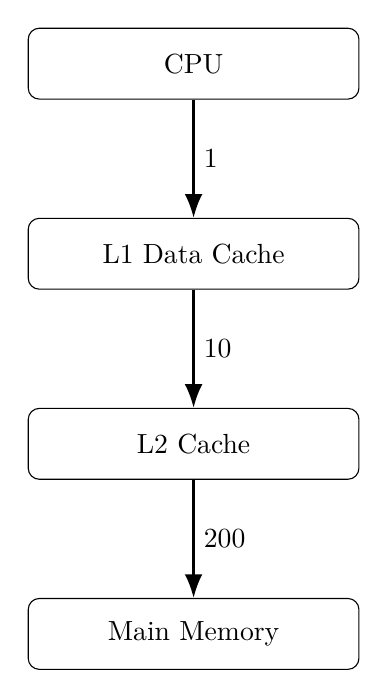
\begin{tikzpicture}[
    node distance=1.5cm,
    block/.style={draw, rounded corners, minimum width=4.2cm, minimum height=0.9cm, align=center},
    arrow/.style={-{Latex[length=3mm]}, thick}
]
    \node[block] (cpu) {CPU};
    \node[block, below=of cpu] (l1) {L1 Data Cache};
    \node[block, below=of l1] (l2) {L2 Cache};
    \node[block, below=of l2] (mem) {Main Memory};

    \draw[arrow] (cpu) -- node[right]{1 κύκλος} (l1);
    \draw[arrow] (l1) -- node[right]{10 κύκλοι} (l2);
    \draw[arrow] (l2) -- node[right]{200 κύκλοι} (mem);
\end{tikzpicture}
\end{center}

Η L1 παραμένει σταθερή σε όλα τα πειράματα, με χωρητικότητα 32 KB, 4-way συσχετιστικότητα και block size 32 B. Αντίθετα, η L2 μεταβάλλεται στην Ενότητα 4.2 και κρατείται σε συγκεκριμένες επιλεγμένες διαμορφώσεις στην Ενότητα 4.3. Οι καθυστερήσεις που χρησιμοποιούνται είναι:

\begin{table}[htbp]
\centering
\caption{Καθυστερήσεις του μοντέλου προσομοίωσης.}
\label{tab:latencies}
\begin{tabular}{lc}
\toprule
\textbf{Περίπτωση πρόσβασης} & \textbf{Καθυστέρηση} \\
\midrule
L1 hit & 1 κύκλος \\
L2 hit & 10 κύκλοι \\
Πρόσβαση στην κύρια μνήμη & 200 κύκλοι \\
\bottomrule
\end{tabular}
\end{table}

Κάθε δυναμική εντολή συνεισφέρει έναν βασικό κύκλο εκτέλεσης. Οι εντολές που προσπελαύνουν δεδομένα στη μνήμη επιβαρύνονται επιπλέον ανάλογα με το επίπεδο της ιεραρχίας στο οποίο εξυπηρετείται η πρόσβαση. Έτσι, το μοντέλο κύκλων που χρησιμοποιείται είναι:

\[
\text{Cycles} = \text{Instructions}
+ \text{L1\_Accesses}\cdot 1
+ \text{L2\_Accesses}\cdot 10
+ \text{Mem\_Accesses}\cdot 200.
\]

Στο συγκεκριμένο μοντέλο κάθε L2 miss οδηγεί σε πρόσβαση στην κύρια μνήμη. Επομένως, οι L2 misses έχουν ιδιαίτερα μεγάλη βαρύτητα στην τελική επίδοση, επειδή αντιστοιχούν σε προσπελάσεις κόστους 200 κύκλων.

\subsection{Μετρικές αξιολόγησης}

Η κύρια μετρική επίδοσης είναι το IPC:

\[
\text{IPC} = \frac{\text{Total Instructions}}{\text{Total Cycles}}.
\]

Η μετρική αυτή αποτυπώνει πόσες εντολές ολοκληρώνονται ανά κύκλο. Στο πλαίσιο της παρούσας άσκησης, υψηλότερο IPC σημαίνει καλύτερη επίδοση.

Για την ανάλυση της συμπεριφοράς της ιεραρχίας μνήμης χρησιμοποιούνται επίσης τα miss rates:

\[
\text{L1 miss rate} = \frac{\text{L1 misses}}{\text{L1 accesses}},
\qquad
\text{L2 miss rate} = \frac{\text{L2 misses}}{\text{L2 accesses}}.
\]

Ωστόσο, το miss rate δεν αρκεί πάντα για πλήρη ερμηνεία, επειδή δεν κανονικοποιεί ως προς τον αριθμό εντολών. Για τον λόγο αυτό χρησιμοποιείται και το MPKI:

\[
\text{L1 MPKI} = \frac{\text{L1 misses}}{\text{Total Instructions}}\cdot 1000,
\qquad
\text{L2 MPKI} = \frac{\text{L2 misses}}{\text{Total Instructions}}\cdot 1000.
\]

Ιδιαίτερα το L2 MPKI είναι κρίσιμη μετρική για την παρούσα άσκηση, επειδή περιγράφει πόσο συχνά, ανά χίλιες εντολές, η εκτέλεση οδηγείται στην ακριβή πρόσβαση της κύριας μνήμης.

\subsection{Αριθμητικός μέσος IPC και aggregate IPC}

Στους πίνακες και στα διαγράμματα εμφανίζονται δύο τρόποι σύνοψης του IPC. Ο αριθμητικός μέσος IPC δίνει ίσο βάρος σε κάθε benchmark:

\[
\overline{\text{IPC}} = \frac{1}{N}\sum_{i=1}^{N}\text{IPC}_i.
\]

Αντίθετα, το \textlatin{aggregate IPC} υπολογίζεται από τα συνολικά instructions και τους συνολικούς κύκλους όλων των benchmarks:

\[
\text{Aggregate IPC} =
\frac{\sum_i \text{Instructions}_i}{\sum_i \text{Cycles}_i}.
\]

Η δεύτερη μορφή είναι πιο κοντά σε σταθμισμένη συνολική επίδοση, επειδή benchmarks με περισσότερους κύκλους ή περισσότερες εντολές επηρεάζουν περισσότερο το τελικό αποτέλεσμα. Για τις τελικές επιλογές της παρούσας αναφοράς δίνεται μεγαλύτερη έμφαση στο aggregate IPC, ενώ ο αριθμητικός μέσος χρησιμοποιείται συμπληρωματικά για να φανεί η συμπεριφορά χωρίς στάθμιση μεταξύ benchmarks.

\section{Πειραματική Μεθοδολογία}

\subsection{Μετροπρογράμματα}

Οι προσομοιώσεις εκτελέστηκαν στα επτά μετροπρογράμματα της εκφώνησης. Ο Πίνακας~\ref{tab:benchmarks} παρουσιάζει συνοπτικά το σύνολο αξιολόγησης.

\begin{table}[htbp]
\centering
\caption{Μετροπρογράμματα που χρησιμοποιήθηκαν στις προσομοιώσεις.}
\label{tab:benchmarks}
\begin{tabular}{cl}
\toprule
\textbf{Α/Α} & \textbf{Benchmark} \\
\midrule
1 & \texttt{403.gcc} \\
2 & \texttt{429.mcf} \\
3 & \texttt{433.milc} \\
4 & \texttt{444.namd} \\
5 & \texttt{450.soplex} \\
6 & \texttt{459.GemsFDTD} \\
7 & \texttt{470.lbm} \\
\bottomrule
\end{tabular}
\end{table}

Η εκτέλεση έγινε αυτοματοποιημένα, ώστε κάθε συνδυασμός παραμέτρων να δοκιμάζεται με τον ίδιο τρόπο. Τα παραγόμενα αρχεία εξόδου αναλύθηκαν σε CSV summaries και ελέγχθηκαν για ελλιπείς ή μη αναγνώσιμες εκτελέσεις.

\subsection{Έλεγχος πληρότητας πειραμάτων}

Για την Ενότητα 4.2 εκτελέστηκαν 21 διαμορφώσεις L2 σε 7 benchmarks, δηλαδή συνολικά 147 προσομοιώσεις. Για την Ενότητα 4.3 εκτελέστηκαν 4 επιλεγμένες L2 διαμορφώσεις, 6 πολιτικές αντικατάστασης και 7 benchmarks, δηλαδή συνολικά 168 προσομοιώσεις. Και στις δύο περιπτώσεις όλα τα outputs αναλύθηκαν επιτυχώς.

\begin{table}[htbp]
\centering
\caption{Πληρότητα εκτελέσεων πειραμάτων.}
\label{tab:validation}
\begin{tabular}{lccc}
\toprule
\textbf{Ενότητα} & \textbf{Αναμενόμενα outputs} & \textbf{Parsed outputs} & \textbf{Missing/unparseable} \\
\midrule
4.2 - Μελέτη χαρακτηριστικών L2 & 147 & 147 & 0 \\
4.3 - Πολιτικές αντικατάστασης & 168 & 168 & 0 \\
\bottomrule
\end{tabular}
\end{table}

Επιπλέον, τα stderr logs των εκτελέσεων ήταν κενά και δεν καταγράφηκαν μη μηδενικοί κωδικοί επιστροφής. Συνεπώς, τα αποτελέσματα που χρησιμοποιούνται στην αναφορά βασίζονται σε πλήρες σύνολο επιτυχημένων προσομοιώσεων.

\section{Μελέτη Χαρακτηριστικών της L2 Cache}

\subsection{Χώρος σχεδίασης}

Στην Ενότητα 4.2 διατηρήθηκε σταθερή η L1 cache και μεταβλήθηκαν μόνο τα χαρακτηριστικά της L2. Η πολιτική αντικατάστασης ήταν LRU σε όλες τις εκτελέσεις αυτού του μέρους. Ο χώρος σχεδίασης που εξετάστηκε φαίνεται στον Πίνακα~\ref{tab:l2-design-space}.

\begin{table}[htbp]
\centering
\caption{Χώρος σχεδίασης L2 cache για την Ενότητα 4.2.}
\label{tab:l2-design-space}
\begin{tabular}{ccc}
\toprule
\textbf{L2 size (KB)} & \textbf{L2 associativity} & \textbf{L2 block size (B)} \\
\midrule
256 & 4 & 64, 128, 256 \\
512 & 4, 8, 16 & 64, 128, 256 \\
1024 & 8, 16 & 64, 128, 256 \\
2048 & 16 & 64, 128, 256 \\
\bottomrule
\end{tabular}
\end{table}

Ο συνολικός αριθμός διαμορφώσεων είναι 21. Για κάθε διαμόρφωση καταγράφηκαν οι κύκλοι, οι προσπελάσεις και τα misses στα επίπεδα L1 και L2, και από αυτά υπολογίστηκαν IPC, miss rates και MPKI.

\subsection{Συνολική κατάταξη διαμορφώσεων}

Το Σχήμα~\ref{fig:42-ranked} παρουσιάζει την κατάταξη των διαμορφώσεων με βάση το aggregate IPC. Παρατηρείται ότι οι καλύτερες διαμορφώσεις έχουν όλες block size 256 B. Αυτό είναι το πιο έντονο μοτίβο της Ενότητας 4.2: για τα συγκεκριμένα benchmarks, το μεγαλύτερο block size αξιοποιεί σημαντικά τη χωρική τοπικότητα και μειώνει τον αριθμό ακριβών L2 misses.

\begin{figure}[htbp]
\centering
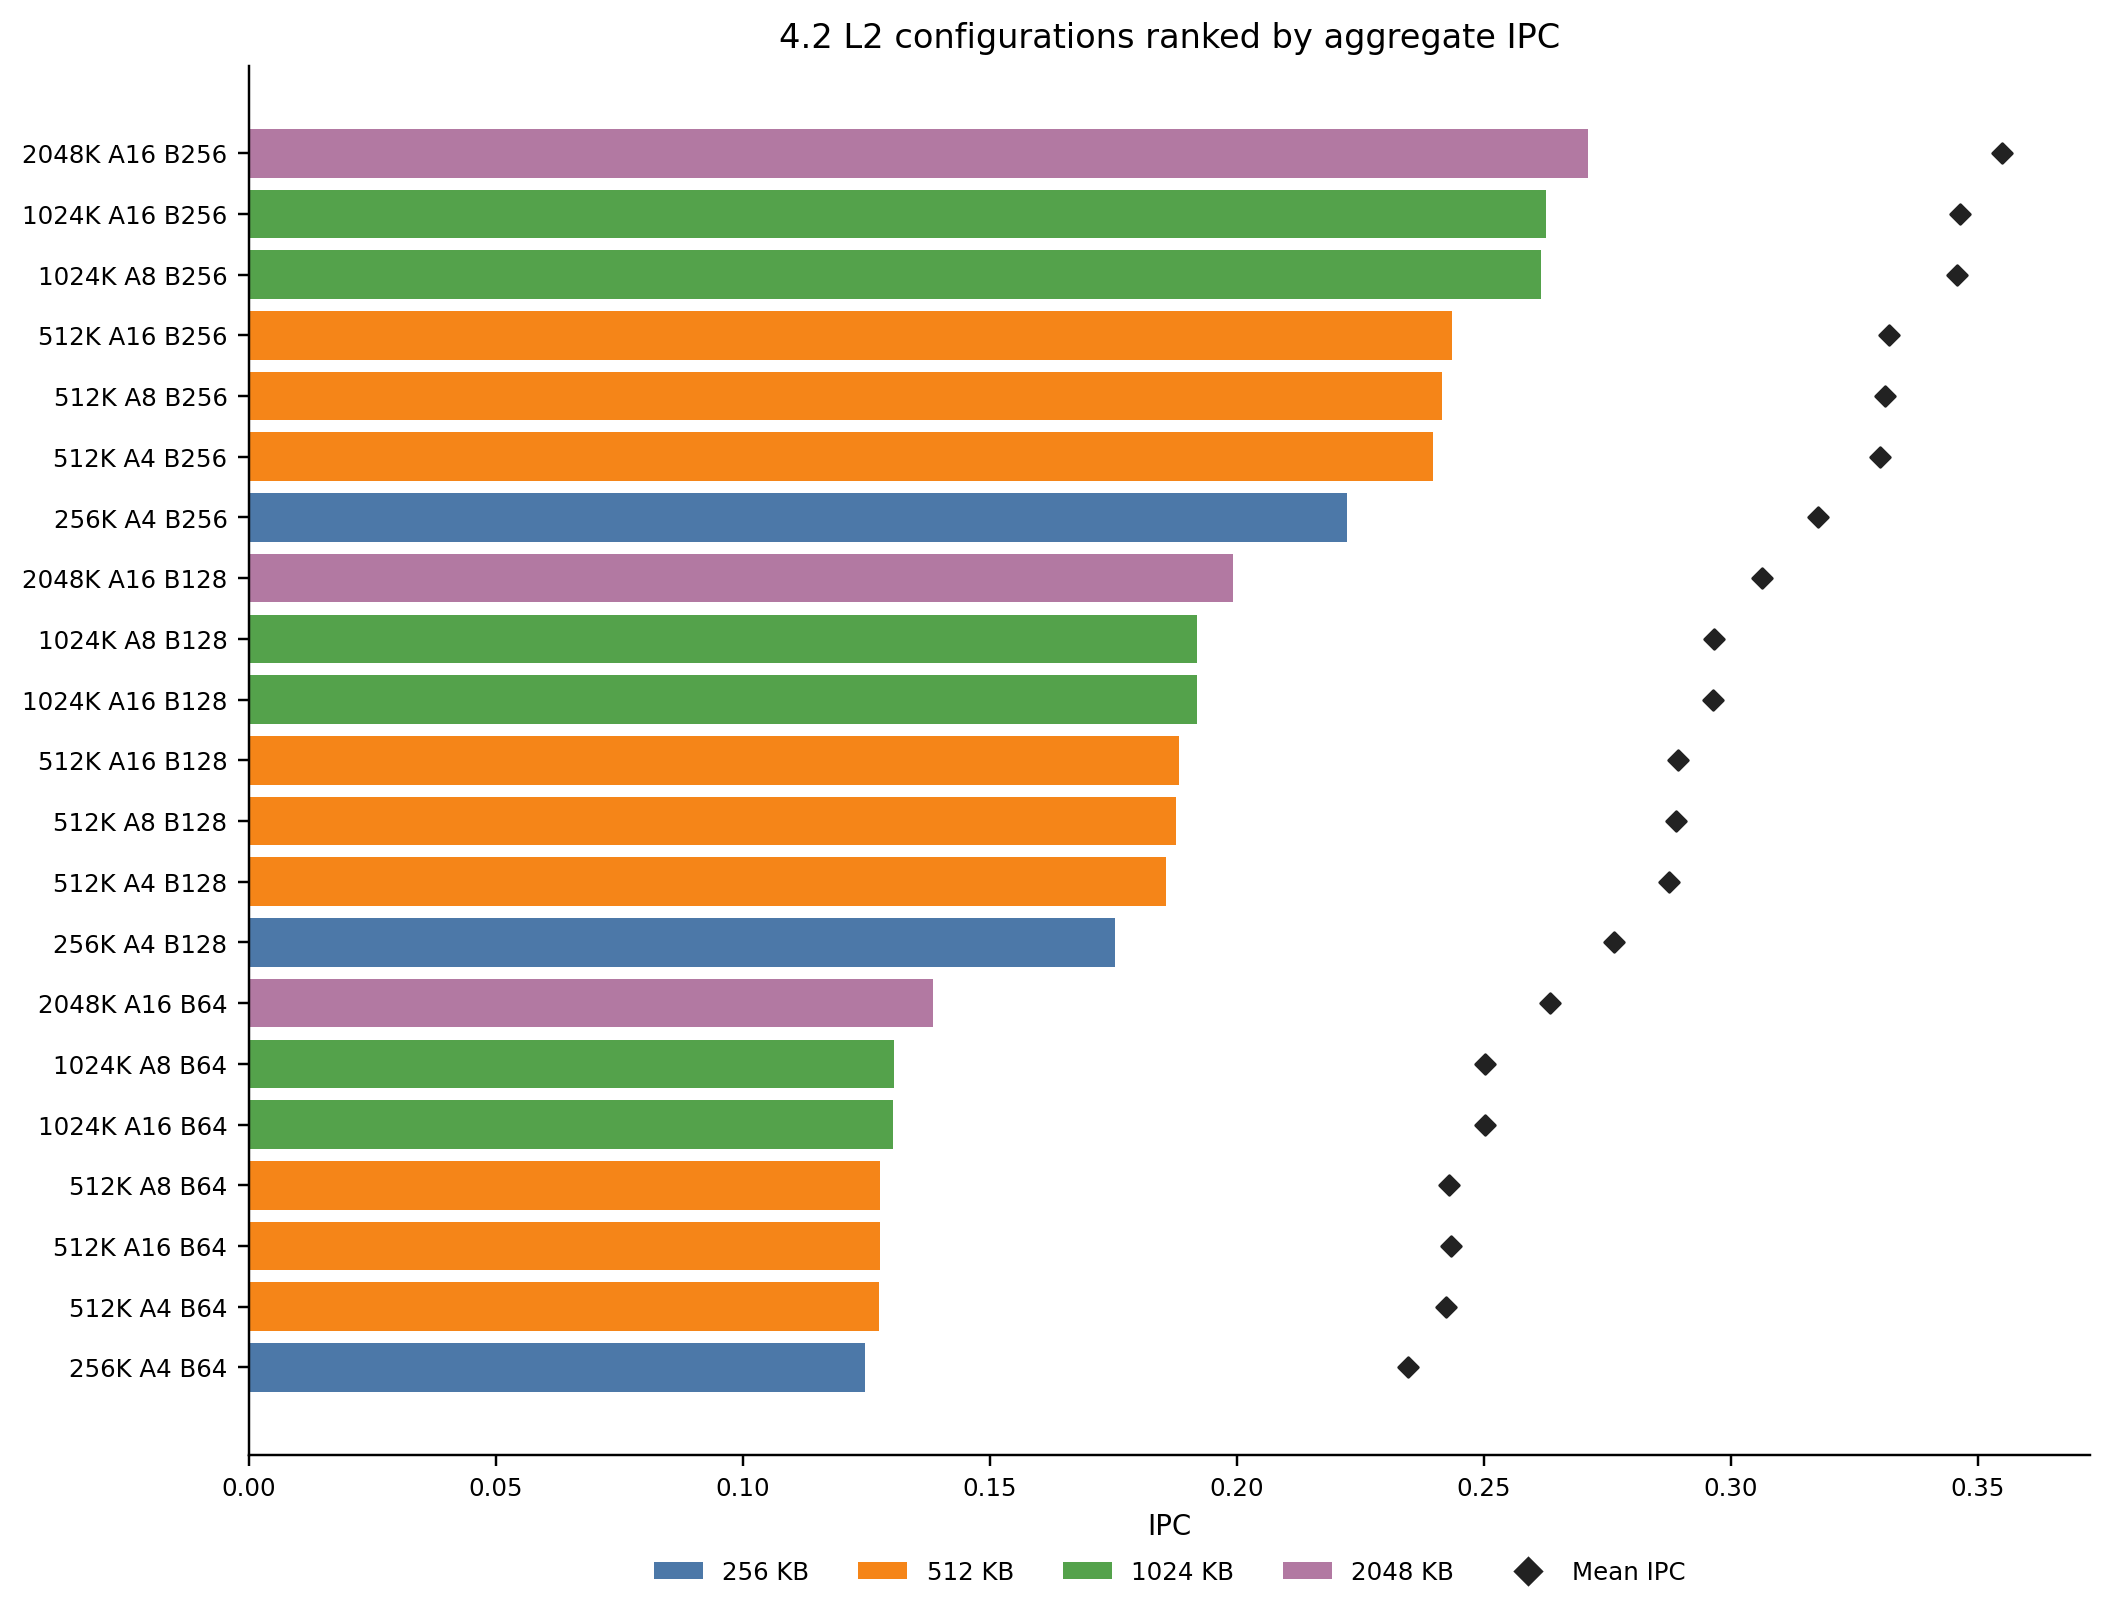
\includegraphics[width=0.93\textwidth]{4_2_config_ipc_ranked.png}
\caption{Κατάταξη των L2 διαμορφώσεων της Ενότητας 4.2 με βάση το aggregate IPC. Τα διαμάντια δείχνουν τον αριθμητικό μέσο IPC.}
\label{fig:42-ranked}
\end{figure}

Η καλύτερη συνολική διαμόρφωση είναι η \texttt{L2\_2048KB\_A16\_B256}, με αριθμητικό μέσο IPC 0.354948, aggregate IPC 0.271145 και aggregate L2 MPKI 8.596625. Η επίδοση αυτή συνδυάζει τη μεγαλύτερη χωρητικότητα, υψηλή συσχετιστικότητα και το μεγαλύτερο block size του χώρου σχεδίασης.

\subsection{Επίδραση του block size}

Το Σχήμα~\ref{fig:42-block-size} απομονώνει την επίδραση του block size, χρησιμοποιώντας για κάθε χωρητικότητα την καλύτερη διαθέσιμη συσχετιστικότητα. Η αύξηση από 64 B σε 128 B και στη συνέχεια σε 256 B βελτιώνει σταθερά το aggregate IPC για όλες τις χωρητικότητες.

\begin{figure}[htbp]
\centering
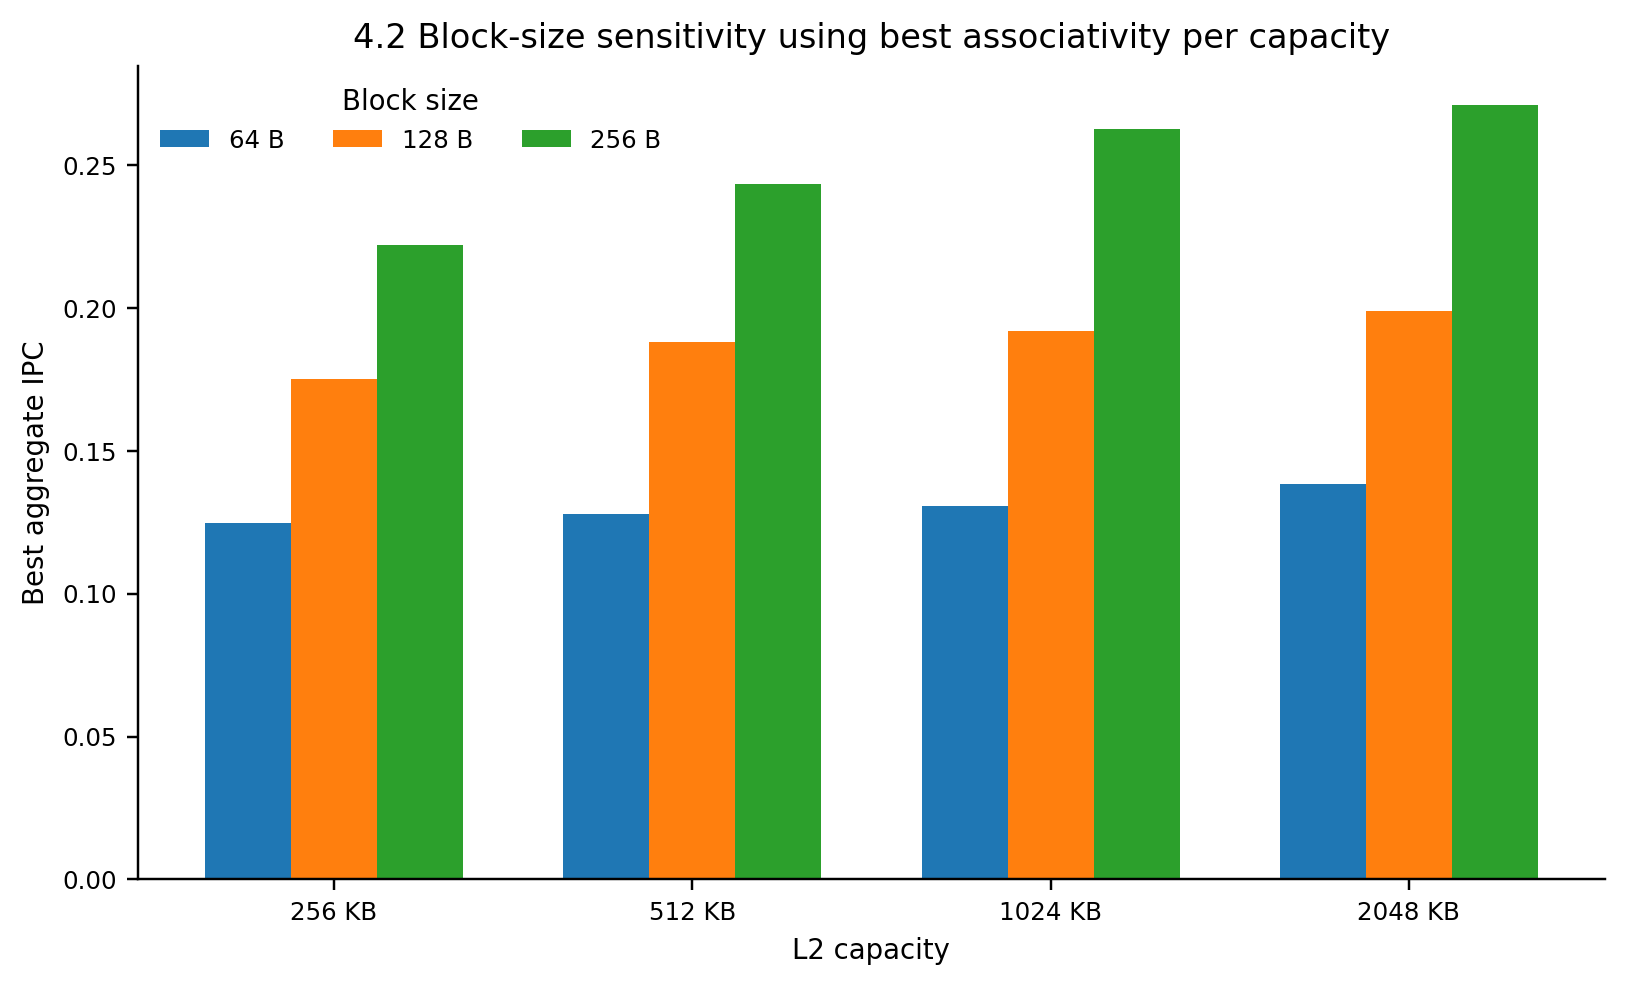
\includegraphics[width=0.9\textwidth]{4_2_block_size_sensitivity.png}
\caption{Ευαισθησία του aggregate IPC ως προς το L2 block size, με χρήση της καλύτερης συσχετιστικότητας ανά χωρητικότητα.}
\label{fig:42-block-size}
\end{figure}

Τα αριθμητικά αποτελέσματα του Πίνακα~\ref{tab:block-sensitivity} δείχνουν ότι η αύξηση του block size είναι η παράμετρος με τη μεγαλύτερη επίδραση στην επίδοση. Για παράδειγμα, στα 2048 KB το aggregate IPC αυξάνεται από 0.138586 με block size 64 B σε 0.271145 με block size 256 B. Παρόμοια ισχυρή βελτίωση παρατηρείται και στις υπόλοιπες χωρητικότητες.

\begin{table}[htbp]
\centering
\caption{Καλύτερο aggregate IPC ανά χωρητικότητα και block size. Για κάθε κελί χρησιμοποιείται η καλύτερη διαθέσιμη συσχετιστικότητα.}
\label{tab:block-sensitivity}
\begin{tabular}{cP{2.7cm}P{2.7cm}P{2.7cm}}
\toprule
\textbf{L2 size} & \textbf{64 B} & \textbf{128 B} & \textbf{256 B} \\
\midrule
256 KB & 0.124686 & 0.175362 & 0.222269 \\
512 KB & 0.127849 & 0.188268 & 0.243580 \\
1024 KB & 0.130574 & 0.191988 & 0.262623 \\
2048 KB & 0.138586 & 0.199160 & 0.271145 \\
\bottomrule
\end{tabular}
\end{table}

Η συμπεριφορά αυτή δείχνει ότι, για τα συγκεκριμένα ίχνη μνήμης, η χωρική τοπικότητα είναι έντονη. Μεγαλύτερα blocks μεταφέρουν περισσότερα γειτονικά δεδομένα ανά miss, με αποτέλεσμα ένα μέρος των επόμενων προσπελάσεων να εξυπηρετείται από την L2 χωρίς νέα πρόσβαση στην κύρια μνήμη. Παρότι μεγάλα blocks μπορούν θεωρητικά να σπαταλήσουν χωρητικότητα ή bandwidth, στο συγκεκριμένο πειραματικό σύνολο το όφελος υπερκαλύπτει το κόστος.

\subsection{Επίδραση της συσχετιστικότητας}

Το Σχήμα~\ref{fig:42-assoc} παρουσιάζει την ευαισθησία ως προς τη συσχετιστικότητα για τις χωρητικότητες όπου υπάρχουν εναλλακτικές τιμές associativity, δηλαδή για 512 KB και 1024 KB. Η επίδραση είναι μικρότερη από αυτή του block size. Για τη χωρητικότητα 512 KB και block size 256 B, το aggregate IPC αυξάνεται από 0.239651 σε 0.243580 όταν η συσχετιστικότητα αυξάνεται από 4-way σε 16-way. Για τη χωρητικότητα 1024 KB και block size 256 B, η αύξηση από 8-way σε 16-way βελτιώνει το aggregate IPC από 0.261541 σε 0.262623.

\begin{figure}[htbp]
\centering
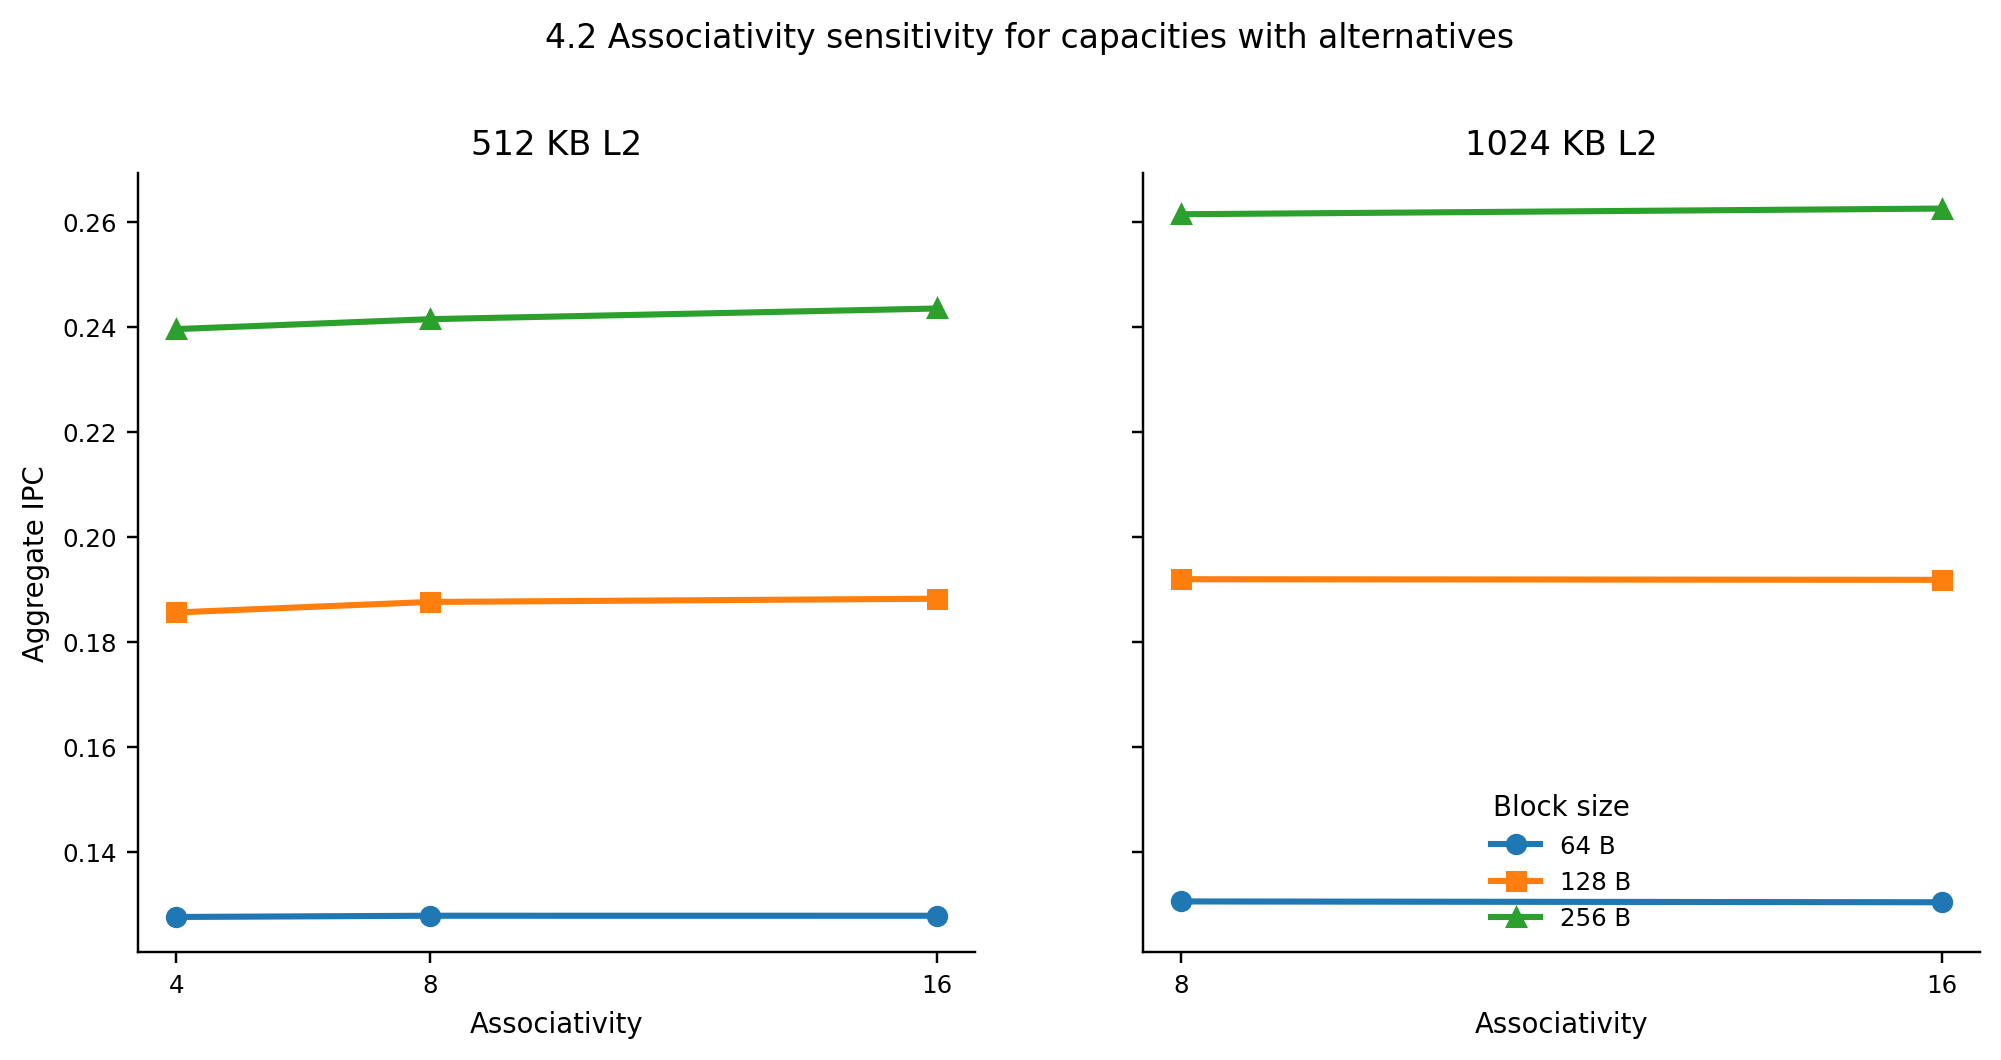
\includegraphics[width=0.93\textwidth]{4_2_associativity_sensitivity.png}
\caption{Ευαισθησία του aggregate IPC ως προς τη συσχετιστικότητα για τις χωρητικότητες 512 KB και 1024 KB.}
\label{fig:42-assoc}
\end{figure}

Το συμπέρασμα είναι ότι η αύξηση της συσχετιστικότητας μειώνει ορισμένα conflict misses, όμως η επίδραση είναι σχετικά περιορισμένη σε σχέση με το block size και τη χωρητικότητα. Αυτό σημαίνει ότι, στο συγκεκριμένο σύνολο μετροπρογραμμάτων, το κυρίαρχο πρόβλημα δεν είναι αποκλειστικά οι συγκρούσεις μέσα στα sets, αλλά κυρίως ο αριθμός ακριβών misses προς την κύρια μνήμη.

\subsection{Επίδραση της χωρητικότητας}

Το Σχήμα~\ref{fig:42-best-capacity} παρουσιάζει την καλύτερη διαμόρφωση για κάθε χωρητικότητα. Η επίδοση βελτιώνεται όσο αυξάνεται η χωρητικότητα της L2, όμως η βελτίωση δεν είναι γραμμική. Η αύξηση από 256 KB σε 512 KB δίνει σαφή βελτίωση, από 0.222269 σε 0.243580 aggregate IPC. Η αύξηση από 512 KB σε 1024 KB συνεχίζει να βελτιώνει την επίδοση, φτάνοντας σε 0.262623. Από 1024 KB σε 2048 KB υπάρχει επιπλέον βελτίωση, αλλά μικρότερη, μέχρι το 0.271145.

\begin{figure}[htbp]
\centering
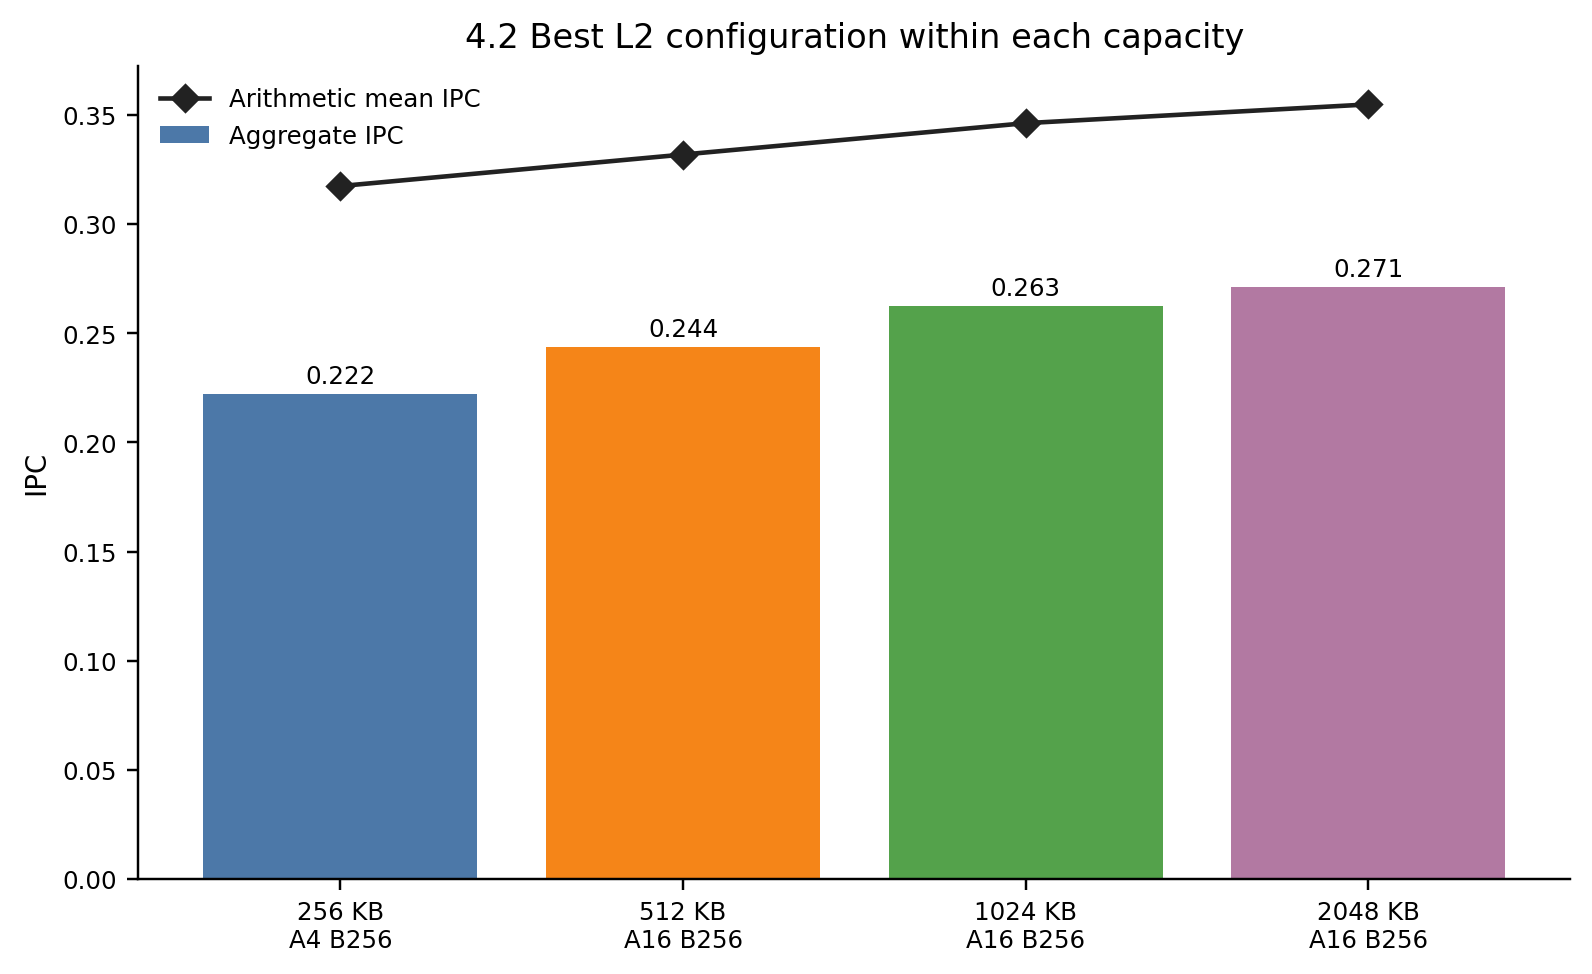
\includegraphics[width=0.85\textwidth]{4_2_best_by_capacity.png}
\caption{Καλύτερη L2 διαμόρφωση εντός κάθε χωρητικότητας. Οι μπάρες δείχνουν aggregate IPC και η γραμμή τον αριθμητικό μέσο IPC.}
\label{fig:42-best-capacity}
\end{figure}

Αυτό είναι αναμενόμενο: η μεγαλύτερη L2 μπορεί να κρατήσει μεγαλύτερο working set και να μειώσει capacity misses, αλλά μετά από κάποιο σημείο μέρος του working set που προκαλεί τα misses δεν χωρά ή δεν επαναχρησιμοποιείται αρκετά γρήγορα ώστε να μετατραπεί σε L2 hits. Έτσι εμφανίζονται φθίνουσες αποδόσεις από την αύξηση χωρητικότητας.

\subsection{Συσχέτιση IPC και L2 MPKI}

Το Σχήμα~\ref{fig:42-mpki-ipc} συγκρίνει το aggregate IPC με το aggregate L2 MPKI. Η σχέση είναι έντονα αρνητική: όσο μειώνεται το L2 MPKI, τόσο αυξάνεται το IPC. Αυτό επιβεβαιώνει ότι η κύρια πηγή διαφοροποίησης της επίδοσης είναι ο αριθμός προσβάσεων στην κύρια μνήμη.

\begin{figure}[htbp]
\centering
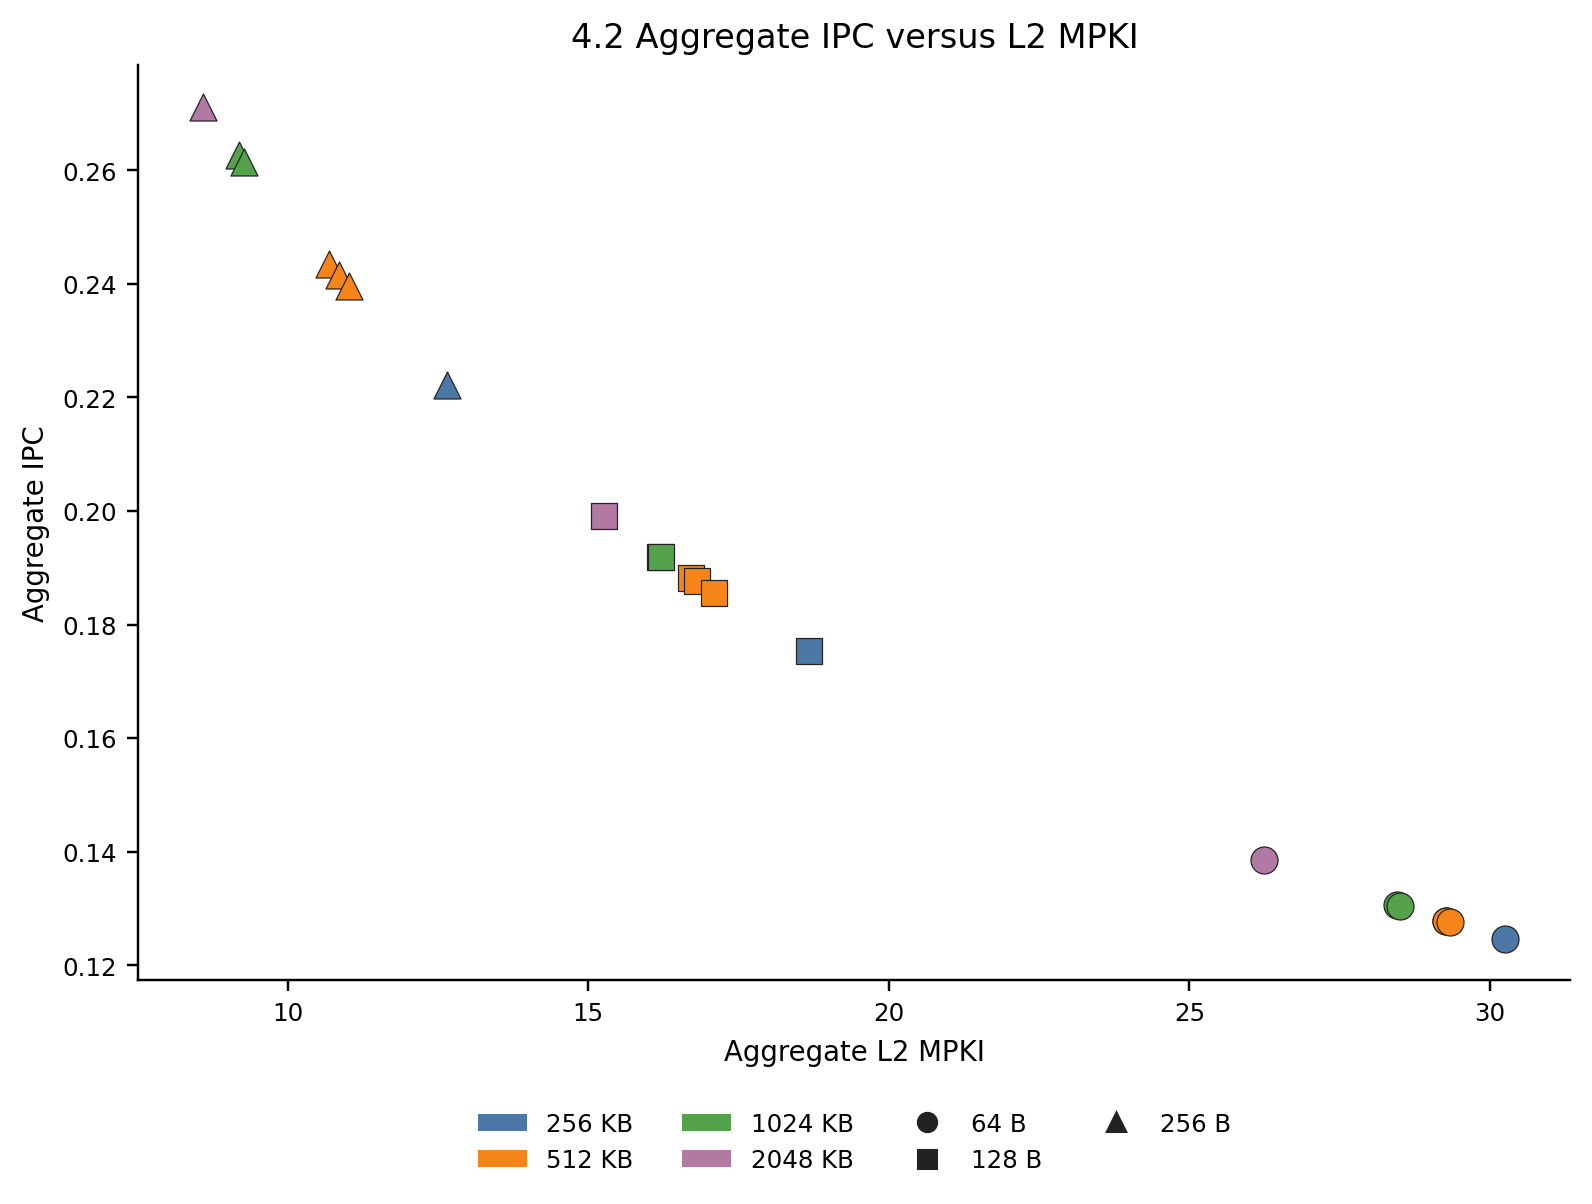
\includegraphics[width=0.85\textwidth]{4_2_l2_mpki_vs_ipc.png}
\caption{Συσχέτιση aggregate IPC και aggregate L2 MPKI για τις διαμορφώσεις της Ενότητας 4.2.}
\label{fig:42-mpki-ipc}
\end{figure}

Οι διαμορφώσεις με block size 64 B βρίσκονται στο δεξί-κάτω μέρος του διαγράμματος, δηλαδή έχουν υψηλό L2 MPKI και χαμηλό IPC. Αντίθετα, οι διαμορφώσεις με block size 256 B βρίσκονται στο αριστερό-πάνω μέρος, δηλαδή έχουν λιγότερα L2 misses ανά χίλιες εντολές και καλύτερη συνολική επίδοση.

\subsection{Συμπεριφορά ανά benchmark}

Το Σχήμα~\ref{fig:42-heatmap} παρουσιάζει το IPC κάθε benchmark για κάθε L2 διαμόρφωση. Η συμπεριφορά δεν είναι ίδια για όλα τα benchmarks. Το \texttt{444.namd} έχει υψηλό IPC σε όλες σχεδόν τις διαμορφώσεις και μικρό εύρος μεταβολής. Αντίθετα, τα \texttt{450.soplex}, \texttt{470.lbm}, \texttt{459.GemsFDTD}, \texttt{433.milc} και \texttt{429.mcf} εμφανίζουν πολύ μεγαλύτερη ευαισθησία στις παραμέτρους της L2.

\begin{figure}[htbp]
\centering
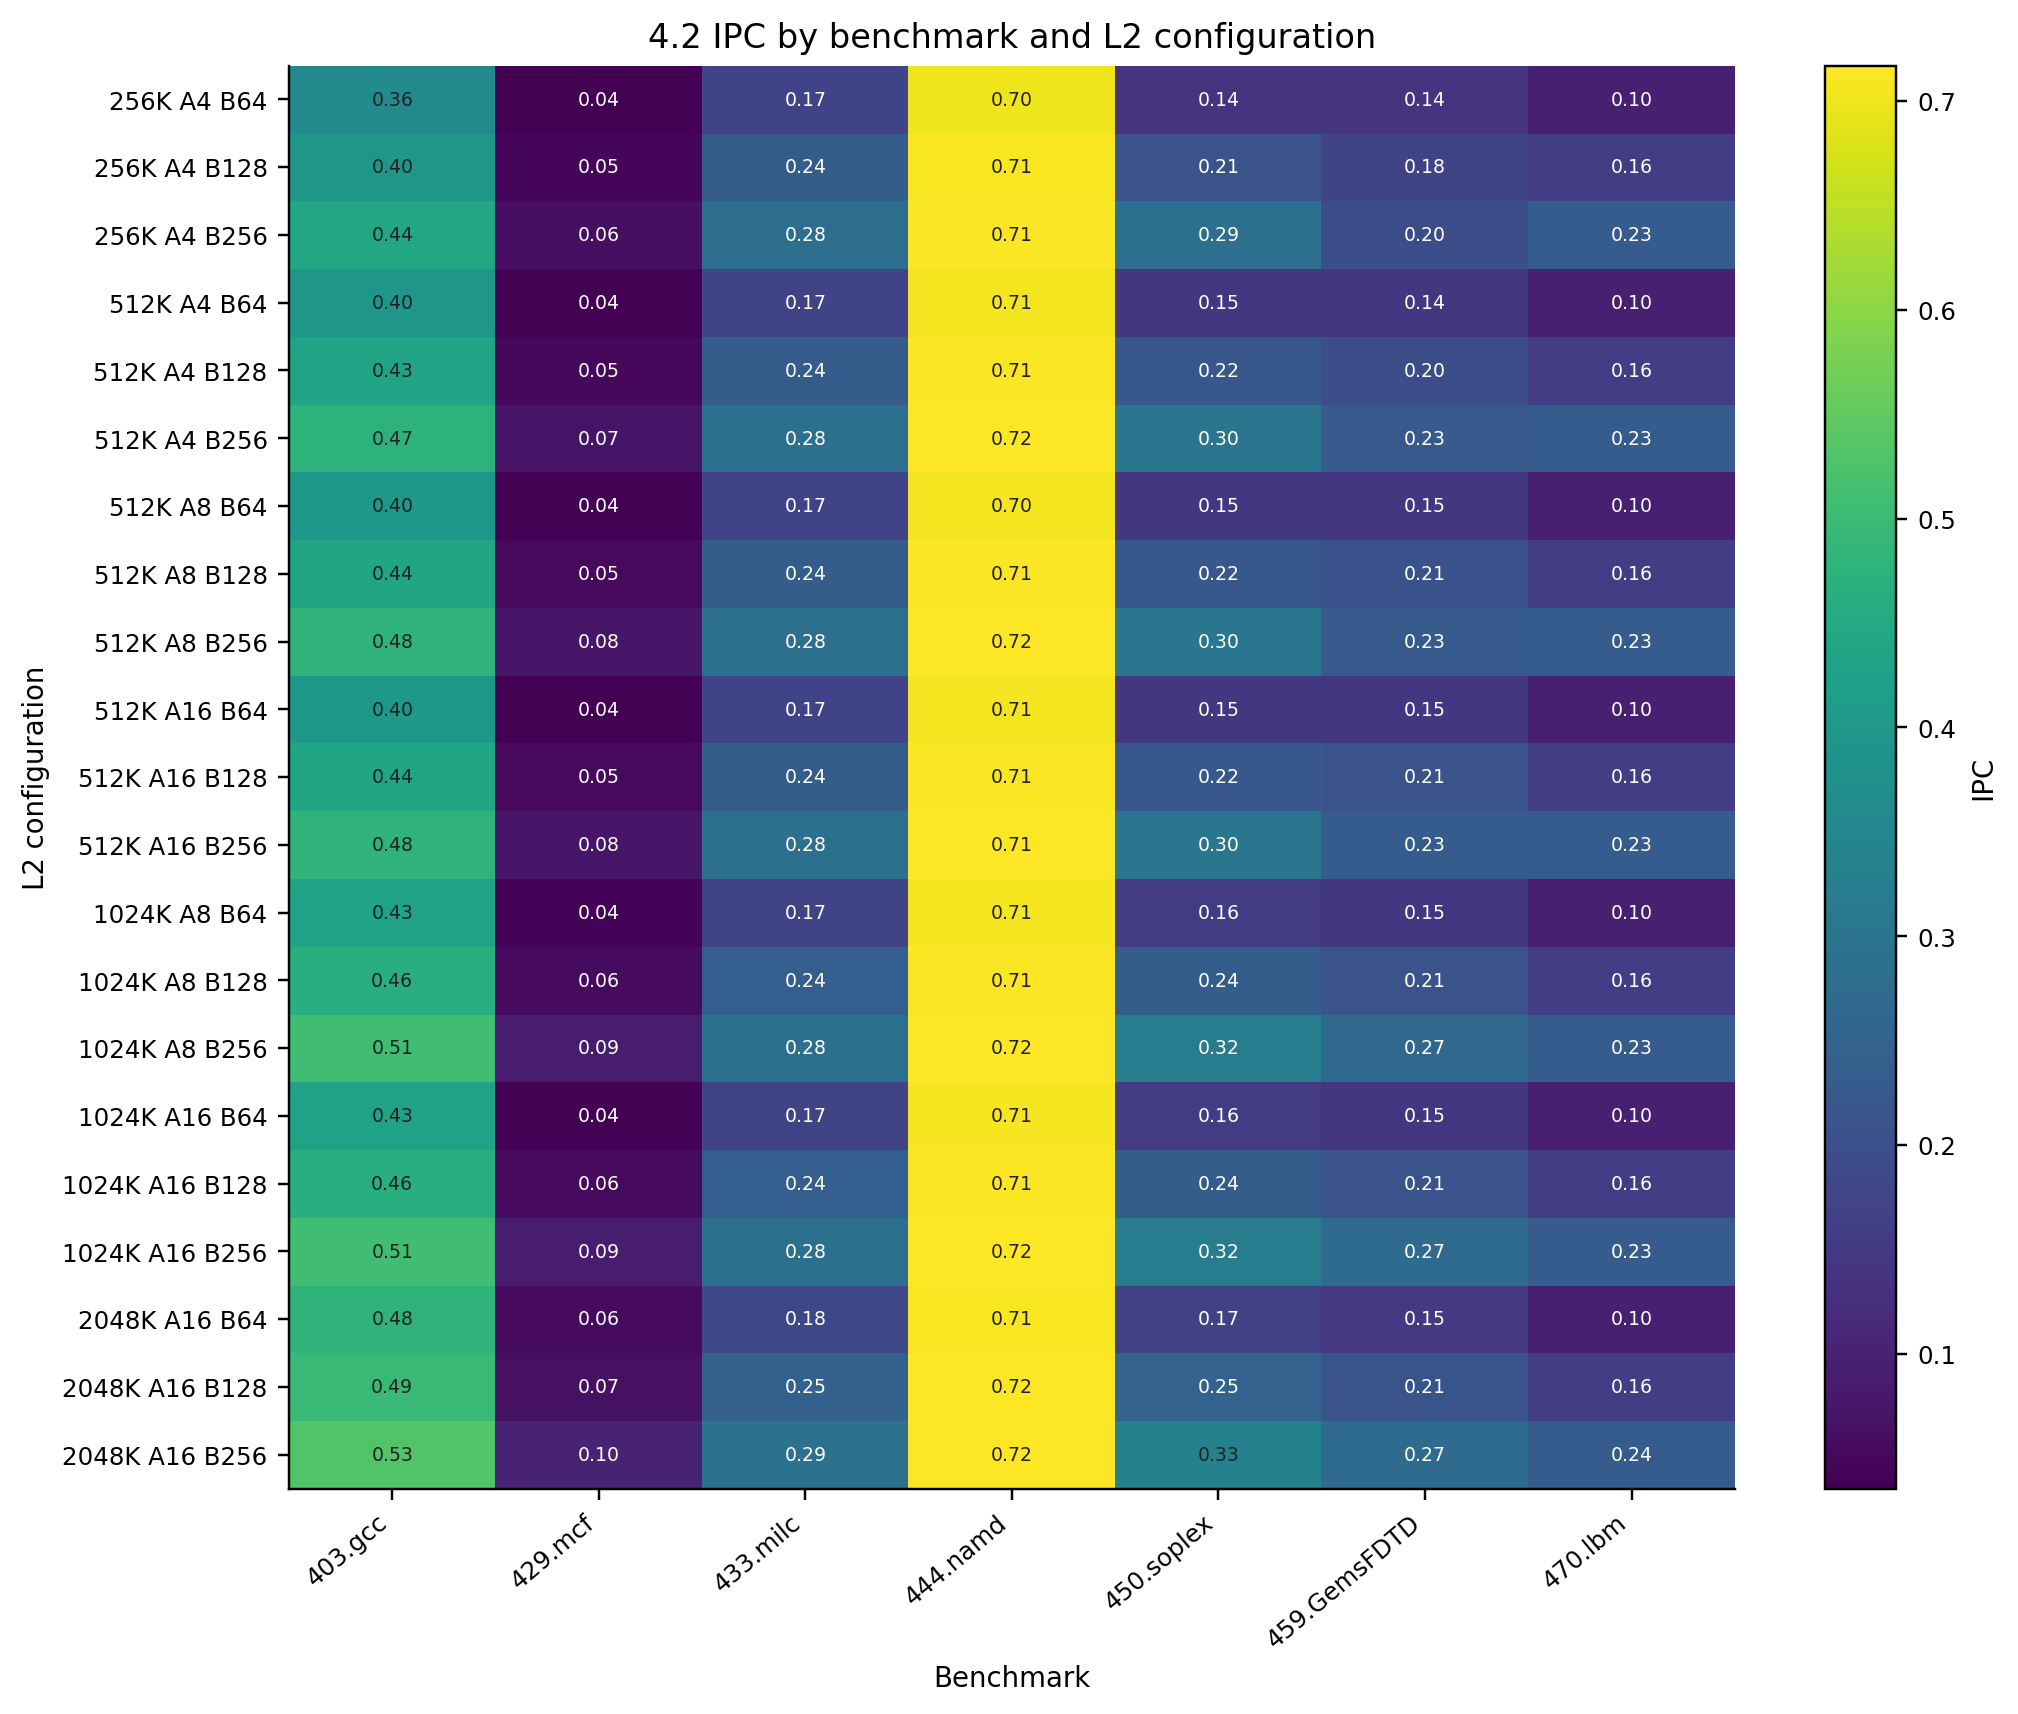
\includegraphics[width=0.92\textwidth]{4_2_benchmark_ipc_heatmap.png}
\caption{IPC ανά benchmark και L2 διαμόρφωση για την Ενότητα 4.2.}
\label{fig:42-heatmap}
\end{figure}

Ο Πίνακας~\ref{tab:benchmark-spread} δείχνει το εύρος μεταβολής IPC ανά benchmark. Το \texttt{444.namd} έχει εύρος μόνο 0.016472, άρα δεν επηρεάζεται έντονα από τις αλλαγές στην L2. Αντίθετα, το \texttt{450.soplex} έχει εύρος 0.193463, το μεγαλύτερο από όλα τα benchmarks, δείχνοντας πολύ μεγαλύτερη εξάρτηση από την ιεραρχία μνήμης.

\begin{table}[htbp]
\centering
\caption{Εύρος μεταβολής IPC ανά benchmark στην Ενότητα 4.2.}
\label{tab:benchmark-spread}
\begin{tabular}{lccc}
\toprule
\textbf{Benchmark} & \textbf{Καλύτερο IPC} & \textbf{Χειρότερο IPC} & \textbf{Εύρος} \\
\midrule
\texttt{403.gcc} & 0.531196 & 0.358763 & 0.172433 \\
\texttt{429.mcf} & 0.103163 & 0.035629 & 0.067534 \\
\texttt{433.milc} & 0.289928 & 0.172253 & 0.117675 \\
\texttt{444.namd} & 0.716906 & 0.700434 & 0.016472 \\
\texttt{450.soplex} & 0.333937 & 0.140474 & 0.193463 \\
\texttt{459.GemsFDTD} & 0.274666 & 0.139235 & 0.135431 \\
\texttt{470.lbm} & 0.235013 & 0.095770 & 0.139243 \\
\bottomrule
\end{tabular}
\end{table}

Από τα παραπάνω φαίνεται ότι τα benchmarks δεν έχουν το ίδιο προφίλ προσβάσεων μνήμης. Όσα παρουσιάζουν υψηλή ευαισθησία ωφελούνται περισσότερο από διαμορφώσεις που μειώνουν το L2 MPKI. Αντίθετα, benchmarks με μικρό εύρος μεταβολής είτε έχουν πιο φιλική συμπεριφορά ως προς την cache είτε δεν περιορίζονται κυρίως από την L2.

\subsection{Βέλτιστη L2 διαμόρφωση ανά χωρητικότητα}

Η εκφώνηση ζητά να επιλεγεί η καλύτερη cache για κάθε διαθέσιμη χωρητικότητα. Με κριτήριο το aggregate IPC, οι επιλογές φαίνονται στον Πίνακα~\ref{tab:best-capacity}.

\begin{table}[htbp]
\centering
\caption{Βέλτιστη L2 διαμόρφωση ανά χωρητικότητα με βάση το aggregate IPC.}
\label{tab:best-capacity}
\begin{tabular}{c l c c c}
\toprule
\textbf{L2 size} & \textbf{Διαμόρφωση} & \textbf{Mean IPC} & \textbf{Aggregate IPC} & \textbf{Aggregate L2 MPKI} \\
\midrule
256 KB & \texttt{L2\_256KB\_A4\_B256} & 0.317521 & 0.222269 & 12.644373 \\
512 KB & \texttt{L2\_512KB\_A16\_B256} & 0.331967 & 0.243580 & 10.681233 \\
1024 KB & \texttt{L2\_1024KB\_A16\_B256} & 0.346354 & 0.262623 & 9.195026 \\
2048 KB & \texttt{L2\_2048KB\_A16\_B256} & 0.354948 & 0.271145 & 8.596625 \\
\bottomrule
\end{tabular}
\end{table}

Και στις τέσσερις χωρητικότητες επιλέγεται block size 256 B. Για τη χωρητικότητα 256 KB υπάρχει μόνο 4-way επιλογή. Για 512 KB και 1024 KB επιλέγεται 16-way, αν και η διαφορά από μικρότερες συσχετιστικότητες είναι περιορισμένη. Για 2048 KB υπάρχει μόνο 16-way επιλογή στον ζητούμενο χώρο σχεδίασης. Συνολικά, αν έπρεπε να επιλεγεί μία διαμόρφωση από όλο το σύνολο της Ενότητας 4.2, η επιλογή θα ήταν η \texttt{L2\_2048KB\_A16\_B256}.

\FloatBarrier

\section{Μελέτη Πολιτικών Αντικατάστασης}

\subsection{Πειραματική διάταξη}

Στην Ενότητα 4.3 χρησιμοποιούνται οι τέσσερις καλύτερες L2 διαμορφώσεις της Ενότητας 4.2, μία για κάθε χωρητικότητα. Για κάθε μία από αυτές εξετάζονται έξι πολιτικές αντικατάστασης: LRU, MRU, Random, LFU, LIP και SRRIP. Σε κάθε προσομοίωση εφαρμόζεται η ίδια πολιτική τόσο στην L1 όσο και στην L2, ώστε η πολιτική αντικατάστασης να είναι η ελεγχόμενη μεταβλητή σε ολόκληρη την ιεραρχία.

Οι πολιτικές που υλοποιήθηκαν και συγκρίθηκαν είναι οι εξής:

\begin{itemize}
    \item \textbf{LRU}: αντικαθιστά το block που χρησιμοποιήθηκε λιγότερο πρόσφατα. Αποτελεί τη baseline πολιτική.
    \item \textbf{MRU}: αντικαθιστά το block που χρησιμοποιήθηκε πιο πρόσφατα. Μπορεί να είναι χρήσιμη σε ορισμένα streaming patterns, αλλά είναι επικίνδυνη όταν υπάρχει ισχυρή χρονική τοπικότητα.
    \item \textbf{Random}: επιλέγει τυχαίο θύμα μέσα στο set. Για την τυχαιότητα χρησιμοποιήθηκε seed 21026, δηλαδή τα πέντε τελευταία ψηφία του ΑΜ.
    \item \textbf{LFU}: κρατά μετρητή χρήσεων για κάθε block και αντικαθιστά αυτό με τη μικρότερη συχνότητα χρήσης. Νέα blocks εισάγονται με μετρητή 1 και σε κάθε hit ο μετρητής αυξάνεται κατά 1.
    \item \textbf{LIP}: έχει ίδια συμπεριφορά με LRU στα hits, αλλά εισάγει τα νέα blocks στη θέση LRU αντί για MRU. Στόχος είναι να προστατεύσει παλαιότερα blocks με αποδεδειγμένη επαναχρησιμοποίηση από blocks που πιθανώς προσπελαύνονται μόνο μία φορά.
    \item \textbf{SRRIP}: χρησιμοποιεί τιμή πρόβλεψης επαναπροσπέλασης για κάθε block. Νέα blocks εισάγονται με τιμή κοντά στο μέγιστο, τα hits θέτουν την τιμή σε 0 και η αντικατάσταση επιλέγει block που προβλέπεται να επαναχρησιμοποιηθεί στο πιο μακρινό μέλλον.
\end{itemize}

\subsection{Συνολική σύγκριση πολιτικών}

Το Σχήμα~\ref{fig:43-overall} παρουσιάζει τη συνολική σύγκριση των πολιτικών ως προς την επίδοση και την πίεση στη μνήμη. Η καλύτερη συνολική πολιτική είναι η LRU, με aggregate IPC 0.248458 και aggregate L2 MPKI 10.278800. Ακολουθούν η Random και η SRRIP. Οι LFU και MRU έχουν σημαντικά χαμηλότερη επίδοση και πολύ υψηλότερο L2 MPKI.

\begin{figure}[htbp]
\centering
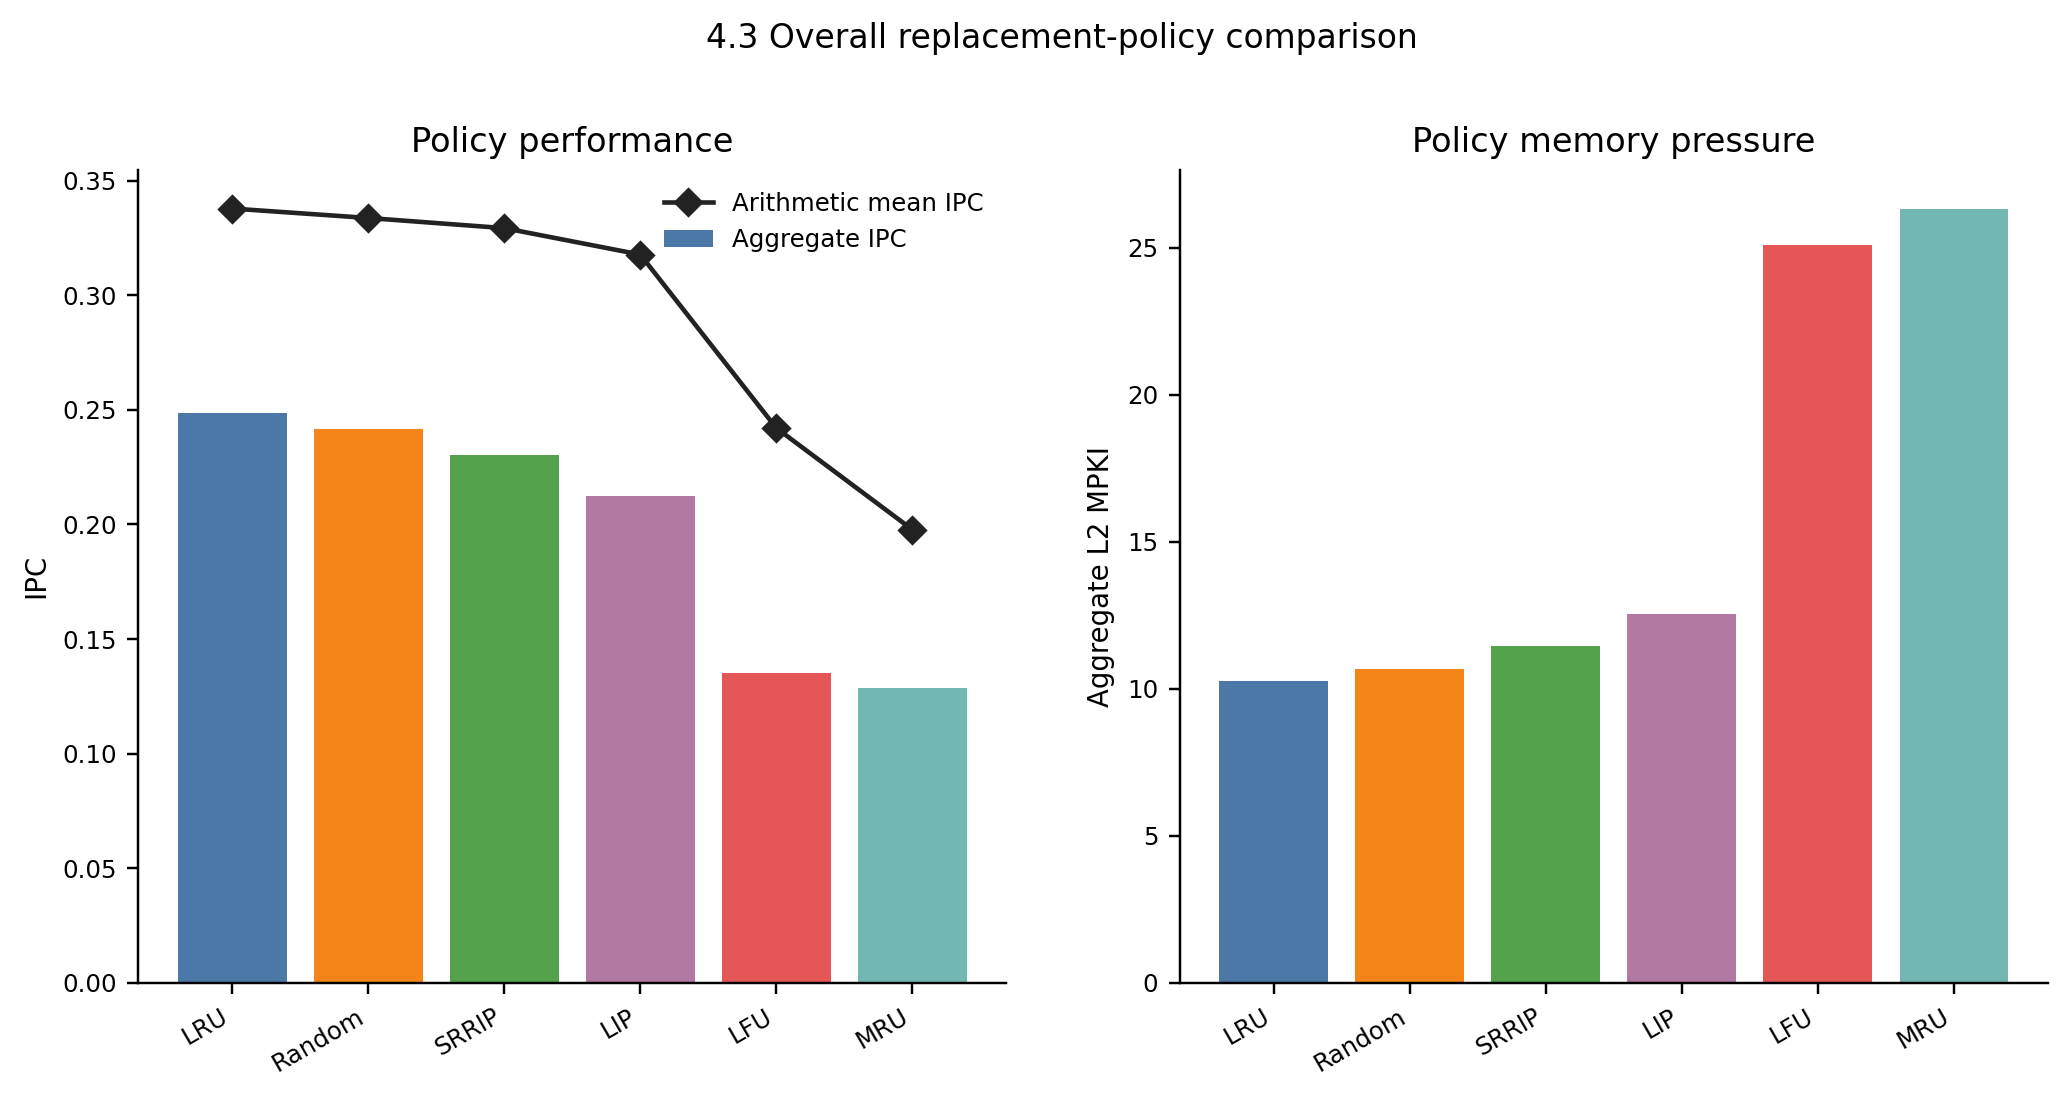
\includegraphics[width=0.93\textwidth]{4_3_policy_overall.png}
\caption{Συνολική σύγκριση πολιτικών αντικατάστασης στην Ενότητα 4.3. Αριστερά παρουσιάζεται η επίδοση και δεξιά το aggregate L2 MPKI.}
\label{fig:43-overall}
\end{figure}

Ο Πίνακας~\ref{tab:policy-overall} δίνει την ίδια κατάταξη αριθμητικά. Η διαφορά LRU και Random είναι σχετικά μικρή, ενώ η διαφορά LRU από LFU και MRU είναι πολύ μεγάλη. Αυτό δείχνει ότι οι πολιτικές που δεν προστατεύουν αποτελεσματικά την πρόσφατη χρονική τοπικότητα δημιουργούν πολλά επιπλέον misses στην L2 και οδηγούν σε περισσότερες ακριβές προσβάσεις στην κύρια μνήμη.

\begin{table}[htbp]
\centering
\caption{Συνολική κατάταξη πολιτικών αντικατάστασης με βάση το aggregate IPC.}
\label{tab:policy-overall}
\begin{tabular}{lcccc}
\toprule
\textbf{Policy} & \textbf{Runs} & \textbf{Mean IPC} & \textbf{Aggregate IPC} & \textbf{Aggregate L2 MPKI} \\
\midrule
LRU & 28 & 0.337797 & 0.248458 & 10.278800 \\
Random & 28 & 0.333681 & 0.241606 & 10.678682 \\
SRRIP & 28 & 0.329256 & 0.230378 & 11.448715 \\
LIP & 28 & 0.317723 & 0.212345 & 12.552042 \\
LFU & 28 & 0.242049 & 0.135381 & 25.104061 \\
MRU & 28 & 0.197742 & 0.128503 & 26.339431 \\
\bottomrule
\end{tabular}
\end{table}

Η LRU λειτουργεί καλύτερα συνολικά επειδή ταιριάζει καλά με workloads που έχουν χρονική τοπικότητα: κρατά τα πρόσφατα χρησιμοποιημένα blocks και απομακρύνει αυτά που έχουν μείνει ανενεργά για περισσότερο χρόνο. Η Random δεν εκμεταλλεύεται άμεσα την τοπικότητα, αλλά αποφεύγει ορισμένες παθολογικές περιπτώσεις και παραμένει σχετικά κοντά στην LRU. Η SRRIP έχει επίσης ανταγωνιστική συμπεριφορά, αλλά στην παρούσα υλοποίηση και στο συγκεκριμένο σύνολο benchmarks δεν ξεπερνά την LRU.

Αντίθετα, η LFU και η MRU αποτυγχάνουν έντονα. Η LFU μπορεί να κρατήσει παλιά blocks με υψηλό μετρητή χρήσεων ακόμη και όταν δεν ανήκουν πλέον στο ενεργό working set. Η MRU, από την άλλη, αντικαθιστά το πιο πρόσφατα χρησιμοποιημένο block, κάτι που είναι επιζήμιο όταν υπάρχει άμεση επαναχρησιμοποίηση.

\subsection{Σύγκριση ανά επιλεγμένη L2 διαμόρφωση}

Το Σχήμα~\ref{fig:43-config-ipc} παρουσιάζει το aggregate IPC κάθε πολιτικής για τις τέσσερις επιλεγμένες L2 διαμορφώσεις. Η γενική εικόνα είναι σταθερή: η LRU βρίσκεται πρώτη στις τρεις μικρότερες χωρητικότητες και η Random είναι οριακά πρώτη στη διαμόρφωση των 2048 KB.

\begin{figure}[htbp]
\centering
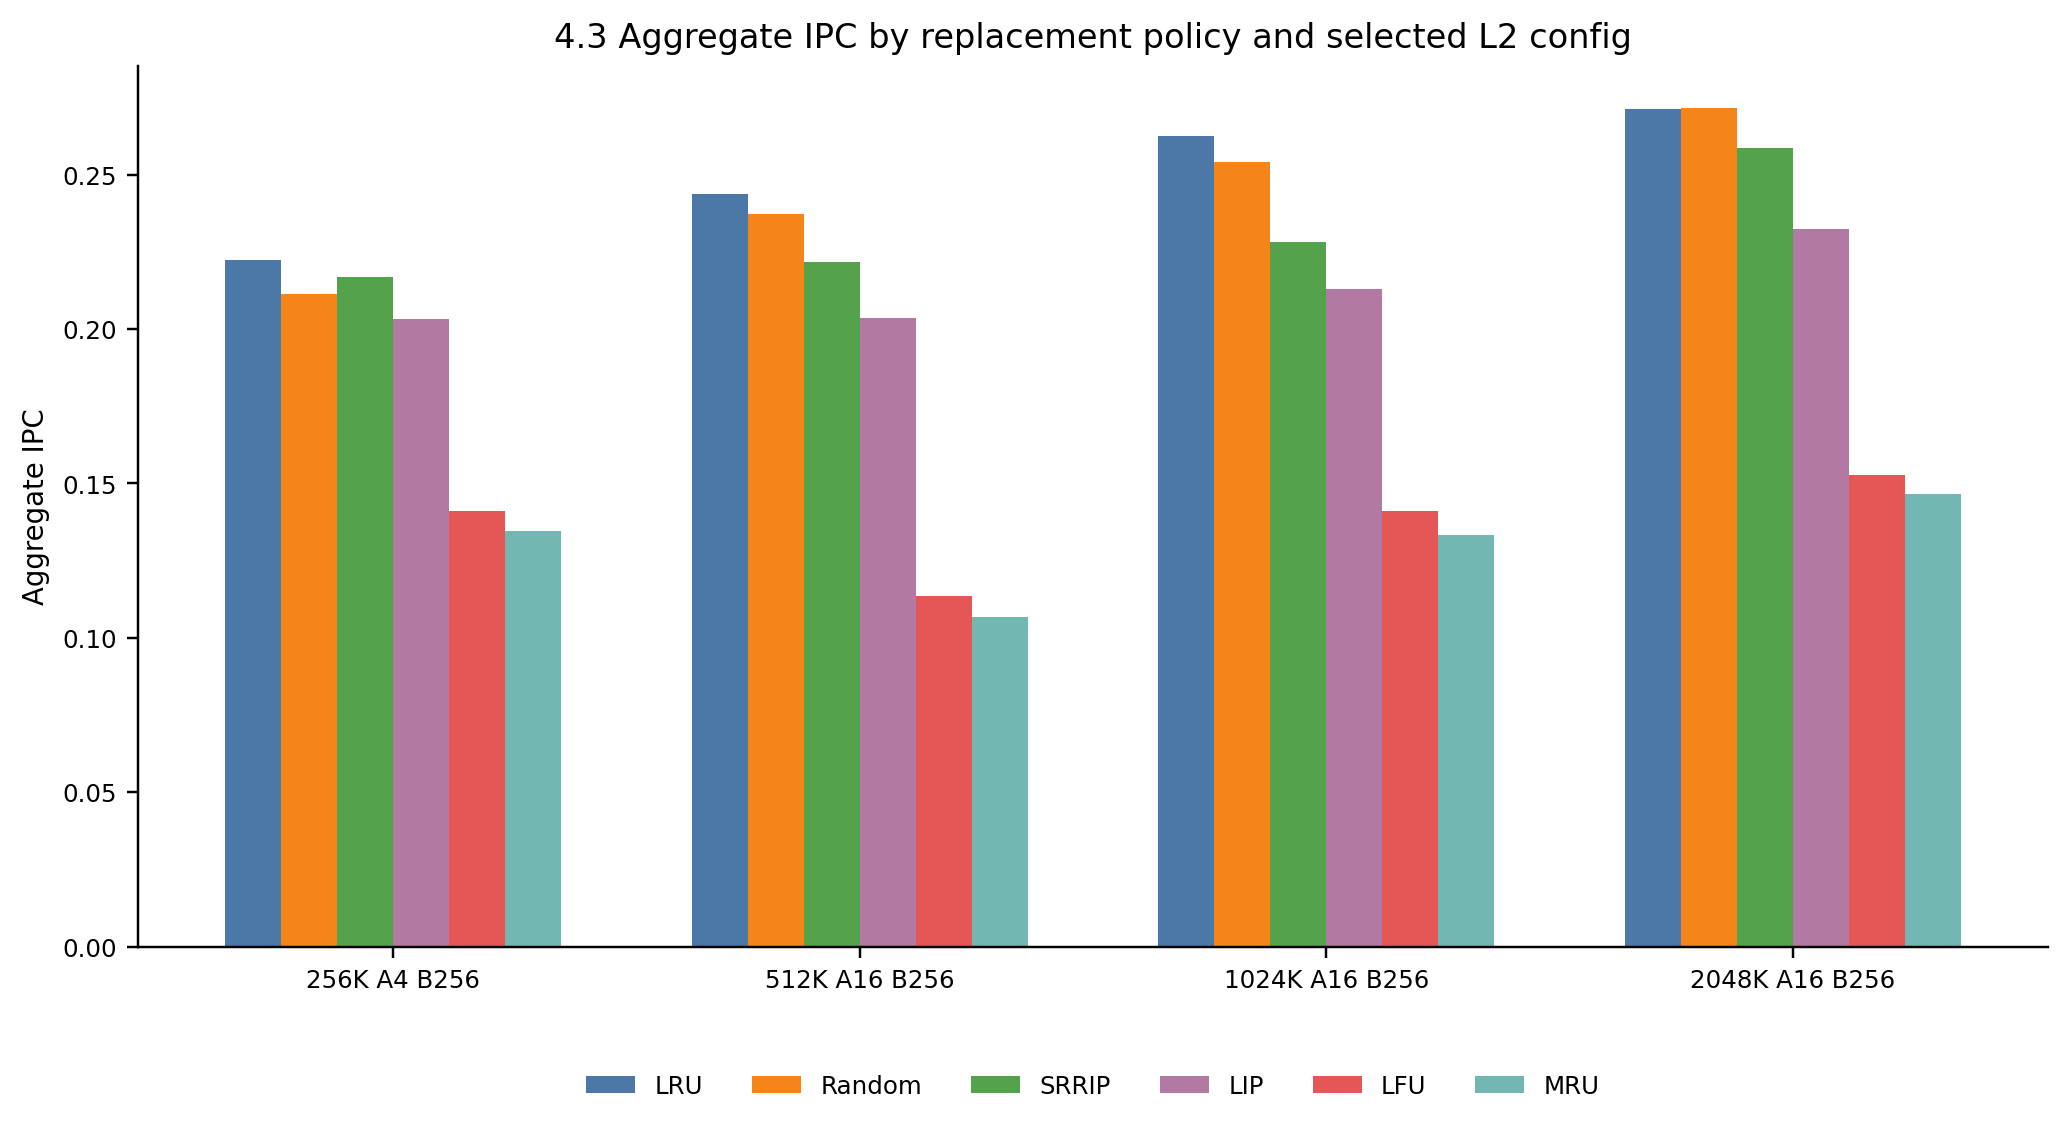
\includegraphics[width=0.9\textwidth]{4_3_policy_by_config_ipc.png}
\caption{Aggregate IPC ανά πολιτική αντικατάστασης και επιλεγμένη L2 διαμόρφωση.}
\label{fig:43-config-ipc}
\end{figure}

Ο Πίνακας~\ref{tab:best-policy-config} συνοψίζει την καλύτερη πολιτική ανά διαμόρφωση. Στις 256 KB, 512 KB και 1024 KB η καλύτερη πολιτική είναι η LRU. Στα 2048 KB η Random έχει aggregate IPC 0.271743, ενώ η LRU έχει 0.271157. Η διαφορά είναι μόλις 0.000586 σε απόλυτο IPC, άρα πρακτικά πρόκειται για πολύ μικρή απόκλιση.

\begin{table}[htbp]
\centering
\caption{Καλύτερη πολιτική αντικατάστασης ανά επιλεγμένη L2 διαμόρφωση.}
\label{tab:best-policy-config}
\begin{tabular}{l c c c c}
\toprule
\textbf{L2 διαμόρφωση} & \textbf{Best policy} & \textbf{Best aggregate IPC} & \textbf{Worst policy} & \textbf{IPC range} \\
\midrule
\texttt{L2\_256KB\_A4\_B256} & LRU & 0.222247 & MRU & 0.087795 \\
\texttt{L2\_512KB\_A16\_B256} & LRU & 0.243643 & MRU & 0.136951 \\
\texttt{L2\_1024KB\_A16\_B256} & LRU & 0.262638 & MRU & 0.129266 \\
\texttt{L2\_2048KB\_A16\_B256} & Random & 0.271743 & MRU & 0.125106 \\
\bottomrule
\end{tabular}
\end{table}

Το Σχήμα~\ref{fig:43-config-mpki} δείχνει το αντίστοιχο aggregate L2 MPKI. Οι πολιτικές LFU και MRU έχουν πολύ υψηλότερο L2 MPKI σε όλες τις χωρητικότητες. Αυτό εξηγεί άμεσα τη χαμηλή επίδοσή τους: οι πρόσθετες L2 misses μεταφράζονται σε περισσότερες προσβάσεις των 200 κύκλων στην κύρια μνήμη.

\begin{figure}[htbp]
\centering
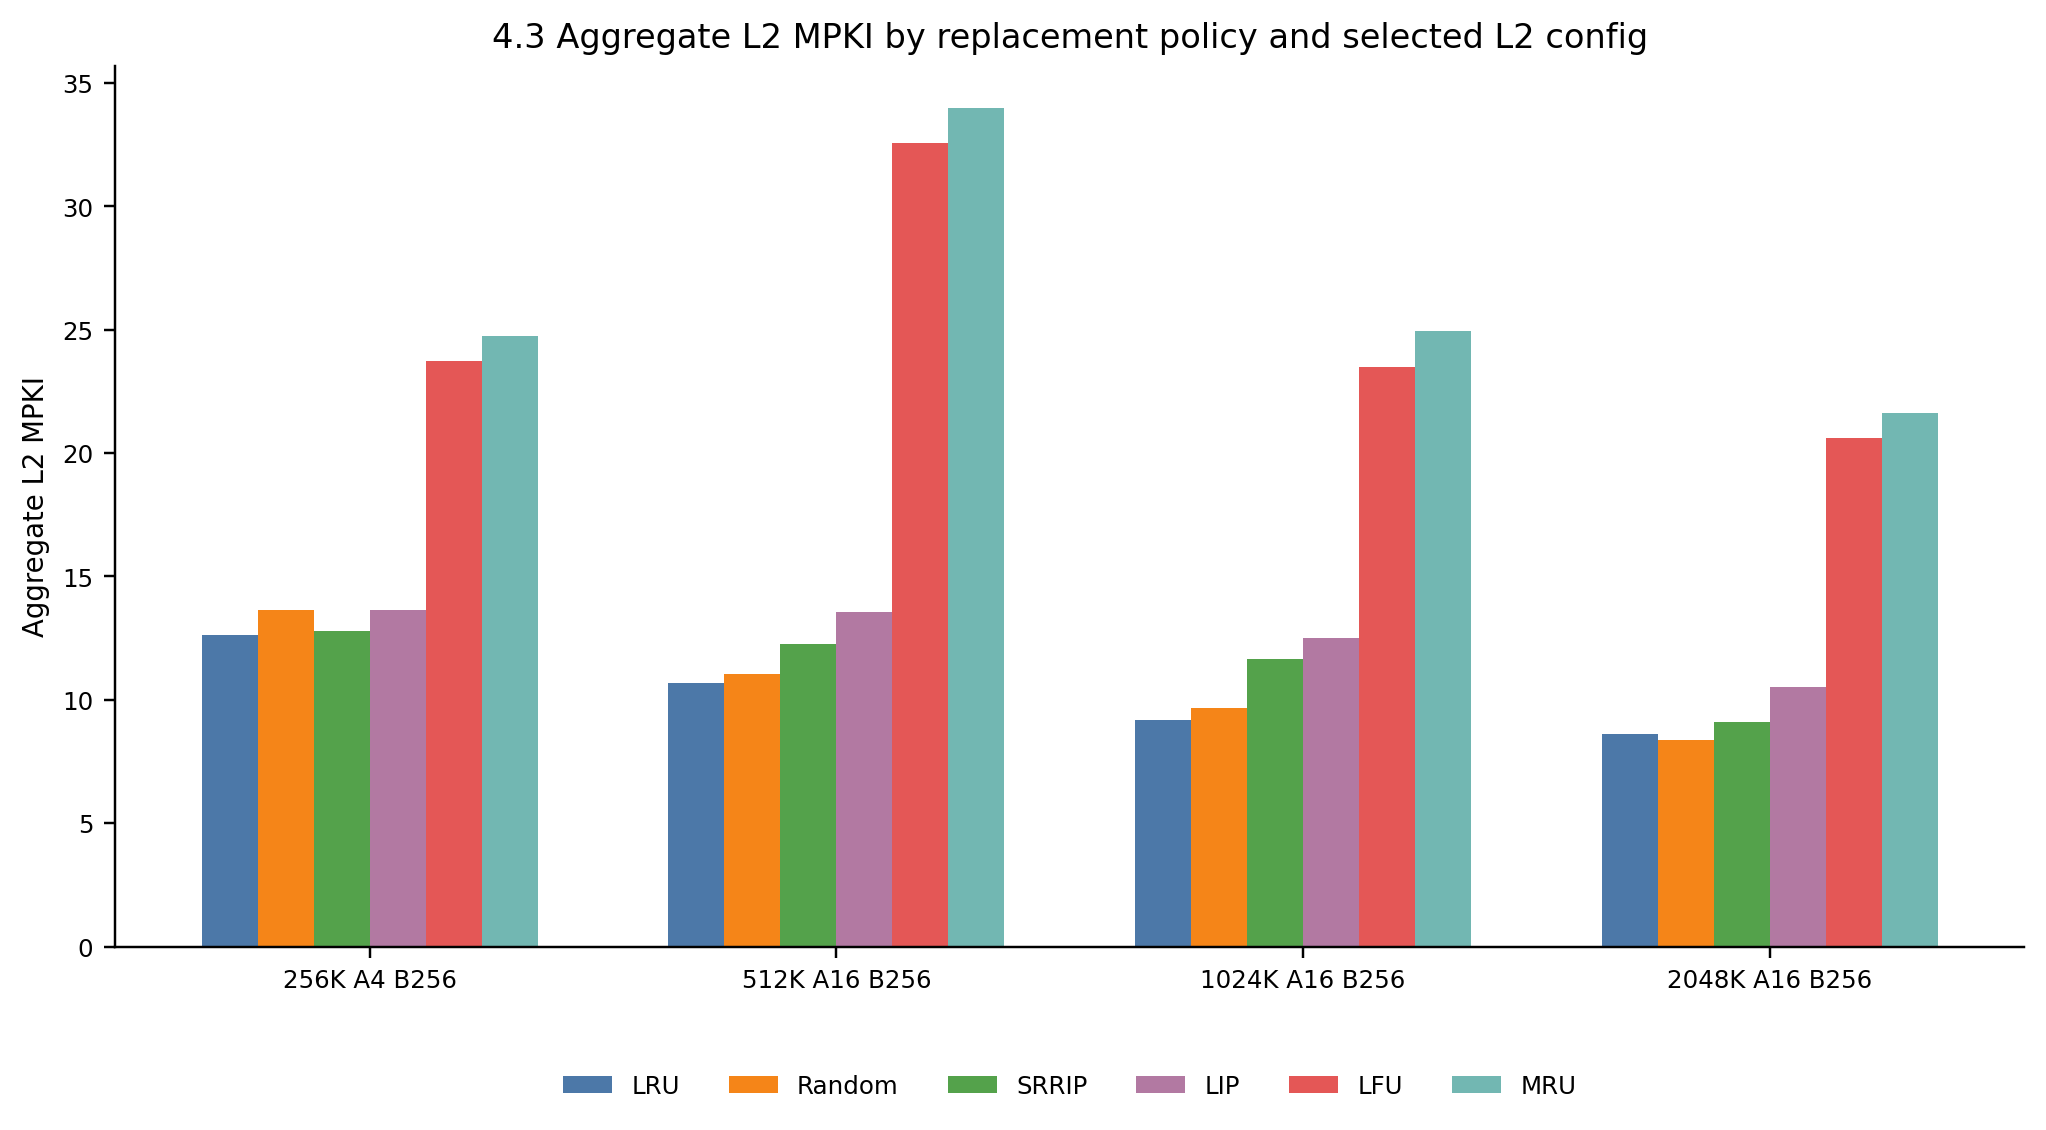
\includegraphics[width=0.9\textwidth]{4_3_policy_by_config_l2_mpki.png}
\caption{Aggregate L2 MPKI ανά πολιτική αντικατάστασης και επιλεγμένη L2 διαμόρφωση.}
\label{fig:43-config-mpki}
\end{figure}

\subsection{Συμπεριφορά ανά benchmark και πολιτική}

Το Σχήμα~\ref{fig:43-policy-benchmark} παρουσιάζει τον μέσο IPC ανά πολιτική και benchmark, υπολογισμένο πάνω στις τέσσερις επιλεγμένες L2 διαμορφώσεις. Η LRU, η Random, η SRRIP και η LIP διατηρούν σχετικά κοντινή συμπεριφορά στα περισσότερα benchmarks, ενώ η LFU και η MRU υποχωρούν αισθητά, ειδικά στα benchmarks που είναι πιο ευαίσθητα στη μνήμη.

\begin{figure}[htbp]
\centering
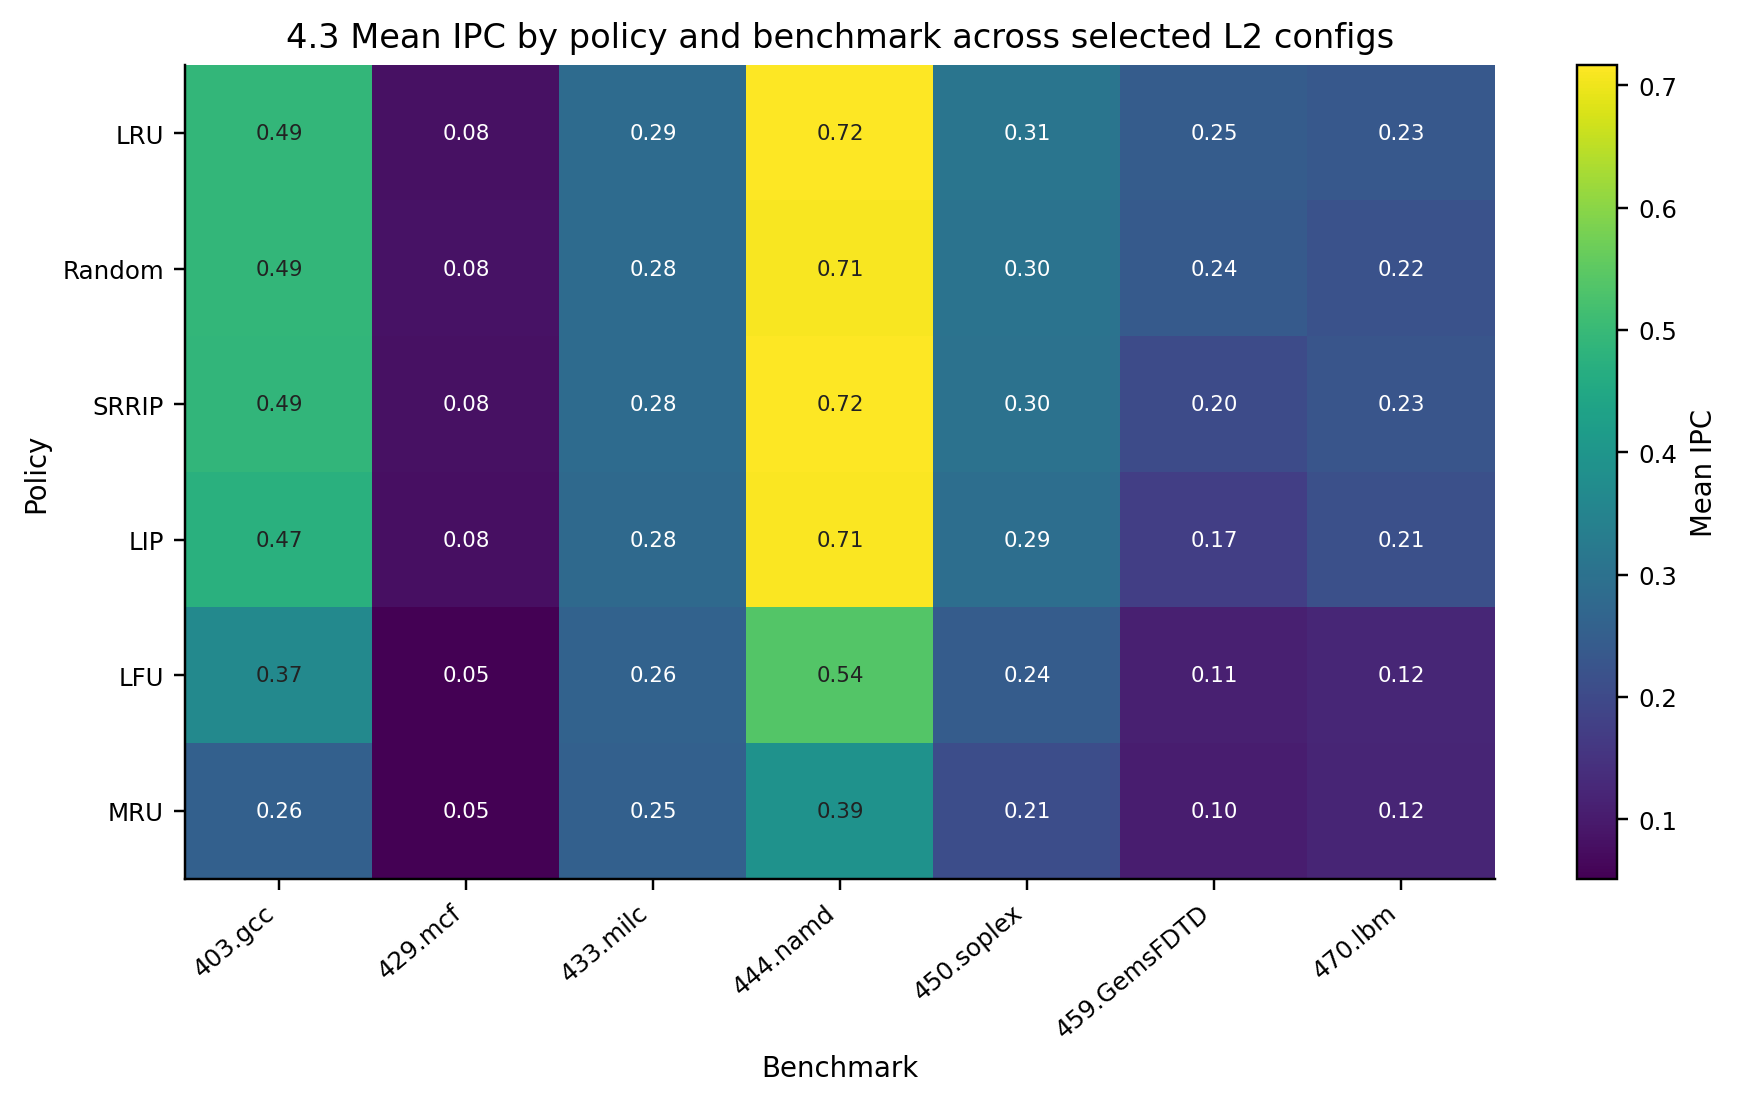
\includegraphics[width=0.9\textwidth]{4_3_policy_benchmark_heatmap.png}
\caption{Μέσο IPC ανά πολιτική αντικατάστασης και benchmark για τις επιλεγμένες L2 διαμορφώσεις.}
\label{fig:43-policy-benchmark}
\end{figure}

Το Σχήμα~\ref{fig:43-random-lru-delta} συγκρίνει ειδικά τη Random με την LRU ανά benchmark. Η Random είναι ελαφρώς καλύτερη σε ορισμένα benchmarks, όπως τα \texttt{403.gcc} και \texttt{429.mcf}, όμως είναι χειρότερη στα περισσότερα υπόλοιπα. Η μεγαλύτερη αρνητική διαφορά εμφανίζεται στο \texttt{470.lbm}. Αυτό εξηγεί γιατί η Random μπορεί να κερδίζει οριακά σε μία συγκεκριμένη διαμόρφωση, αλλά δεν είναι καλύτερη συνολικά από την LRU.

\begin{figure}[htbp]
\centering
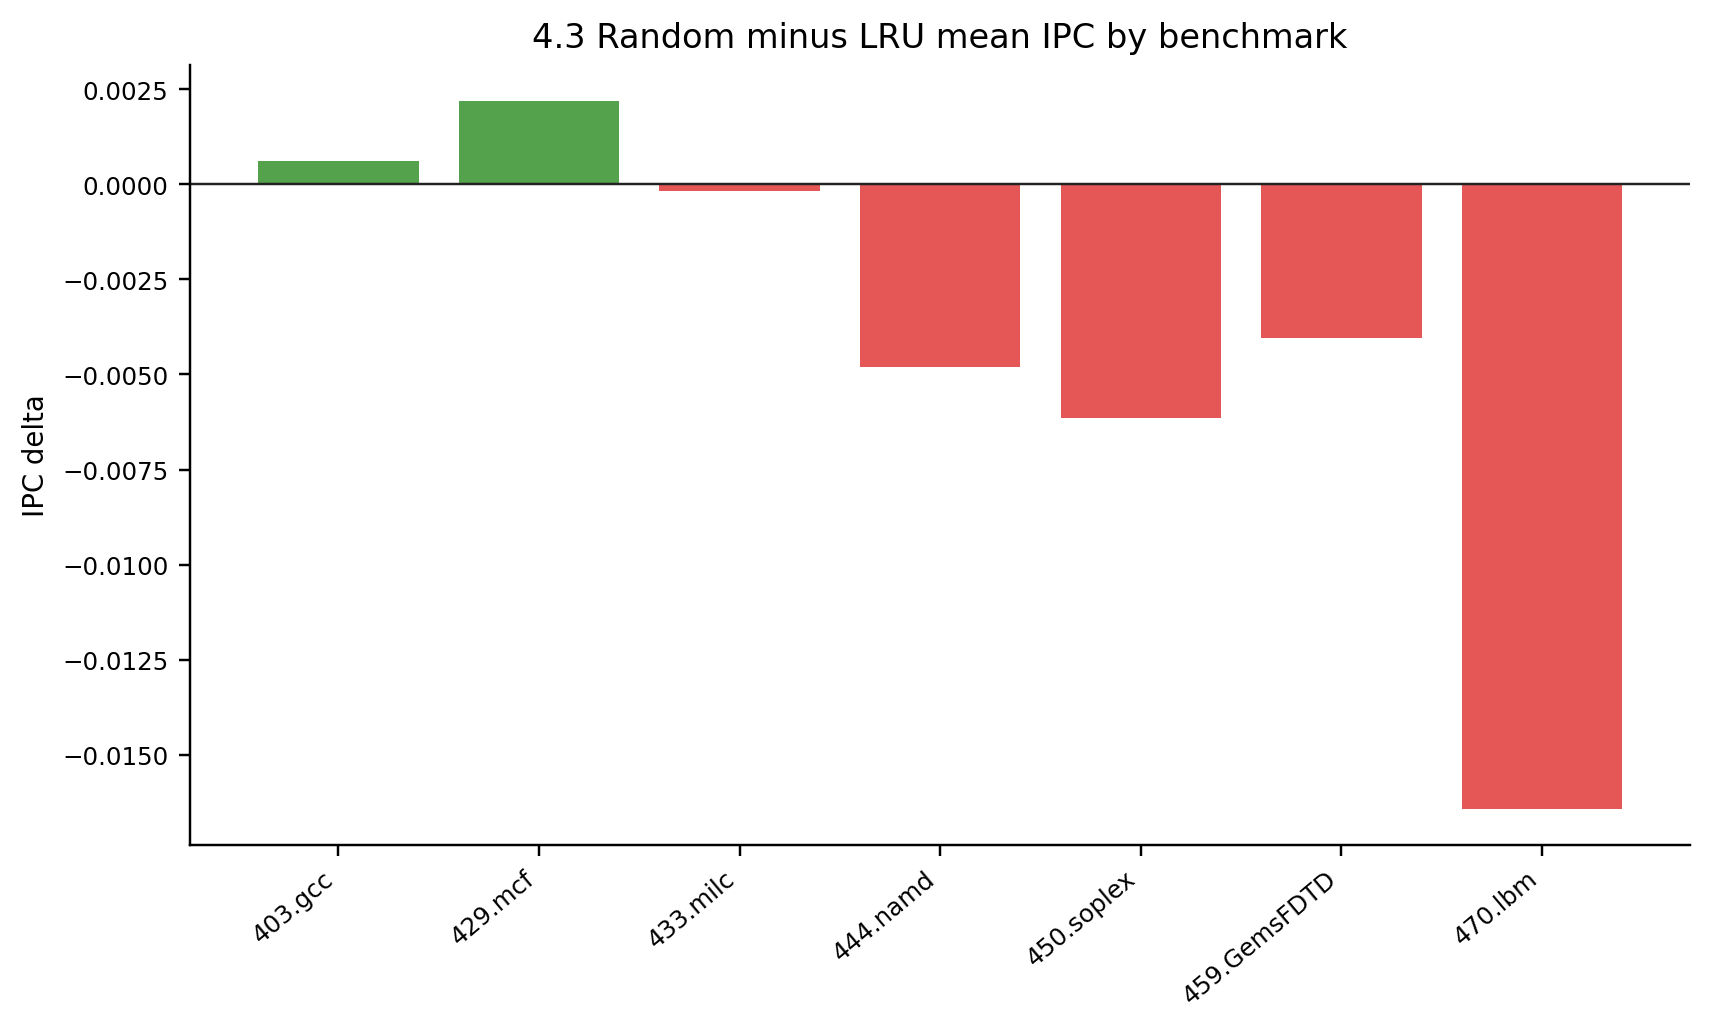
\includegraphics[width=0.9\textwidth]{4_3_lru_random_delta_by_benchmark.png}
\caption{Διαφορά μέσου IPC Random μείον LRU ανά benchmark. Θετικές τιμές σημαίνουν ότι η Random υπερέχει της LRU.}
\label{fig:43-random-lru-delta}
\end{figure}

\subsection{Τελική επιλογή πολιτικής αντικατάστασης}

Με βάση τα συνολικά αποτελέσματα, η πολιτική που θα επιλεγόταν για υλοποίηση στο σύστημα είναι η \textbf{LRU}. Η επιλογή αυτή βασίζεται στους εξής λόγους:

\begin{enumerate}[label=\arabic*)]
    \item Έχει το καλύτερο συνολικό aggregate IPC, ίσο με 0.248458.
    \item Έχει το χαμηλότερο συνολικό aggregate L2 MPKI, ίσο με 10.278800.
    \item Είναι η καλύτερη πολιτική στις τρεις από τις τέσσερις επιλεγμένες L2 διαμορφώσεις.
    \item Στη μοναδική περίπτωση όπου η Random την ξεπερνά, η διαφορά είναι πολύ μικρή σε aggregate IPC.
    \item Έχει σταθερή και ερμηνεύσιμη συμπεριφορά, επειδή προστατεύει αποτελεσματικά την πρόσφατη χρονική τοπικότητα.
\end{enumerate}

Η Random αποτελεί καλή εναλλακτική απλούστερης υλοποίησης, καθώς βρίσκεται κοντά στην LRU και σε μία περίπτωση την ξεπερνά οριακά. Παρ' όλα αυτά, η LRU είναι πιο ασφαλής επιλογή συνολικά, επειδή έχει καλύτερη μέση συμπεριφορά στο σύνολο των benchmarks και των διαμορφώσεων.

\FloatBarrier

\section{Συμπεράσματα}

Η παρούσα άσκηση ανέδειξε τη μεγάλη σημασία της ιεραρχίας μνήμης στην επίδοση εφαρμογών. Παρότι το μοντέλο επεξεργαστή είναι απλοποιημένο, η διαφοροποίηση των κύκλων λόγω L1 hits, L2 hits και προσβάσεων στην κύρια μνήμη αρκεί για να δημιουργήσει μεγάλες διαφορές στο IPC.

Για τη μελέτη της L2 cache στην Ενότητα 4.2, το σημαντικότερο συμπέρασμα είναι ότι το block size είχε τη μεγαλύτερη επίδραση στην επίδοση. Σε όλες τις χωρητικότητες, το block size 256 B ήταν η καλύτερη επιλογή. Αυτό δείχνει ότι τα benchmarks που εξετάστηκαν αξιοποιούν σημαντικά τη χωρική τοπικότητα. Η αύξηση της χωρητικότητας της L2 βελτίωσε επίσης την επίδοση, καθώς μείωσε τα capacity misses, όμως με φθίνουσα απόδοση όσο η χωρητικότητα μεγάλωνε. Η αύξηση της συσχετιστικότητας είχε θετική αλλά πιο περιορισμένη επίδραση.

Οι καλύτερες διαμορφώσεις ανά χωρητικότητα ήταν:

\begin{itemize}
    \item 256 KB: \texttt{L2\_256KB\_A4\_B256},
    \item 512 KB: \texttt{L2\_512KB\_A16\_B256},
    \item 1024 KB: \texttt{L2\_1024KB\_A16\_B256},
    \item 2048 KB: \texttt{L2\_2048KB\_A16\_B256}.
\end{itemize}

Η καλύτερη συνολική διαμόρφωση της Ενότητας 4.2 ήταν η \texttt{L2\_2048KB\_A16\_B256}, με aggregate IPC 0.271145 και aggregate L2 MPKI 8.596625.

Για τη μελέτη πολιτικών αντικατάστασης στην Ενότητα 4.3, η LRU είχε την καλύτερη συνολική συμπεριφορά. Η Random ήταν κοντά και υπερείχε οριακά στη μεγαλύτερη L2 διαμόρφωση, όμως συνολικά είχε χαμηλότερο aggregate IPC από την LRU. Η SRRIP και η LIP είχαν ενδιάμεση συμπεριφορά, ενώ οι LFU και MRU είχαν σημαντικά χειρότερη επίδοση λόγω αυξημένου L2 MPKI.

Συνολικά, για το σύστημα που μελετήθηκε, η πιο ισορροπημένη επιλογή είναι L2 cache 2048 KB, 16-way, block size 256 B, με πολιτική αντικατάστασης LRU. Η επιλογή αυτή συνδυάζει το χαμηλότερο επίπεδο ακριβών προσβάσεων στην κύρια μνήμη με την καλύτερη συνολική επίδοση στο σύνολο των μετροπρογραμμάτων.

\end{document}